\documentclass{beamer}
% \usetheme{default}
\usetheme{Boadilla}
\usepackage[utf8x]{inputenc}
\usepackage{default}
\usepackage{amsmath,amsthm,amsfonts,amssymb,graphicx,xcolor,ifthen}
\usepackage{algorithm,listings}
\usepackage{algorithmicx,algpseudocode}
\usepackage{multirow,array,lscape,chngpage,rotating}
\usepackage{colortbl,calc,fp}

\usepackage{tikz}
\usetikzlibrary{snakes,patterns,shapes,calc}

\usepackage{listings}
\lstloadlanguages{Haskell}

\lstnewenvironment{bigcode}
    %{\lstset{}%
      %\csname lst@SetFirstLabel\endcsname}
    %{\csname lst@SaveFirstLabel\endcsname}
    {
    \lstset{
      %basicstyle=\small\ttfamily,
      basicstyle=\Large\ttfamily,
      xleftmargin=\parindent,
      xleftmargin=\parindent,
      flexiblecolumns=false,
      keepspaces=true,
      %frame=single,
      frame=none,
      basewidth={0.5em,0.45em},
      literate={+}{{$+$}}1 {/}{{$/$}}1 {*}{{$*$}}1 {=}{{$=$}}1
               {>}{{$>$}}1 {<}{{$<$}}1 {\\}{{$\lambda$}}1
               {\\\\}{{\char`\\\char`\\}}1
               {->}{{$\rightarrow$}}2 {>=}{{$\geq$}}2 {<-}{{$\leftarrow$}}2
               {<=}{{$\leq$}}2 {=>}{{$\Rightarrow$}}2
%                {\ .}{{$\circ$}}2 {\ .\ }{{$\circ$}}2
               {>>}{{>>}}2 {>>=}{{>>=}}2
               {|}{{$\mid$}}1
               {<>}{{$\diamond$}}1
               {++}{{$\+$}}1
               {mempty}{{$\epsilon$}}1
               {Theta}{{$\Theta$}}1
    }
    }
    {}

\lstnewenvironment{code}
    %{\lstset{}%
      %\csname lst@SetFirstLabel\endcsname}
    %{\csname lst@SaveFirstLabel\endcsname}
    {
    \lstset{
      basicstyle=\small\ttfamily,
      xleftmargin=\parindent,
      xleftmargin=\parindent,
      flexiblecolumns=false,
      keepspaces=true,
      frame=single,
      basewidth={0.5em,0.45em},
      literate={+}{{$+$}}1 {/}{{$/$}}1 {*}{{$*$}}1 {=}{{$=$}}1
               {>}{{$>$}}1 {<}{{$<$}}1 {\\}{{$\lambda$}}1
               {\\\\}{{\char`\\\char`\\}}1
               {->}{{$\rightarrow$}}2 {>=}{{$\geq$}}2 {<-}{{$\leftarrow$}}2
               {<=}{{$\leq$}}2 {=>}{{$\Rightarrow$}}2
%                {\ .}{{$\circ$}}2 {\ .\ }{{$\circ$}}2
               {>>}{{>>}}2 {>>=}{{>>=}}2
               {|}{{$\mid$}}1
               {<>}{{$\diamond$}}1
               {++}{{$\+$}}1
               {mempty}{{$\epsilon$}}1
               {Theta}{{$\Theta$}}1
    }
    }
    {}
%\tikzstyle{blackbox}=[shape=rectangle, draw, fill=black, text=white, minimum width=0.8in]
\tikzstyle{blackbox}=[shape=rectangle, draw, fill=black, draw=white, draw opacity=0, line width=0.15in, text=white, minimum size=0.3in]
\tikzstyle{whitebox}=[shape=rectangle, draw, fill=white, draw=black, minimum size=0.3in]

%%%%%%%%%%%%%%%%%%%%%%%%%%%%%%%%%%%%%%%
%\newcommand{\h}[1]{\emph{{#1}}}
\newcommand{\h}[1]{\textup{\lstinline{#1}}}
\DeclareMathOperator*{\argmin}{arg\,min}

\newtheoremstyle{nameddefinition}{}{}{}{}{\bfseries}{}{.5em}{#1: \thmnote{#3}.}
\theoremstyle{nameddefinition}
\newtheorem{defn}{Definition}

\newcommand\Algphase[1]{%
\vspace*{-.7\baselineskip}\Statex\hspace*{\dimexpr-\algorithmicindent-2pt\relax}\rule{\textwidth}{0.4pt}%
\Statex\hspace*{-\algorithmicindent}\textbf{#1}%
\vspace*{-.7\baselineskip}\Statex\hspace*{\dimexpr-\algorithmicindent-2pt\relax}\rule{\textwidth}{0.4pt}%
}

\newcommand{\set}[1]{\ensuremath{\mathcal{{#1}}}}
%\newcommand{\vector}[1]{\textbf{{{#1}}}}
\newcommand{\elem}[1]{\textbf{{#1}}}
\newcommand\op{\ensuremath{\diamond}}
\newcommand\id{\ensuremath{\mathbf{\epsilon}}}
\newcommand\+{\op}
%\newcommand\+{\mdoubleplus}
\newcommand\doubleplus{+\kern-1.3ex+\kern0.8ex}
\newcommand\mdoubleplus{\ensuremath{\mathbin{+\mkern-10mu+}}}

\newcommand{\nn}[1]{\ensuremath{\ensuremath{{{#1}}_{nn}}}}
\newcommand{\dist}[2]{\ensuremath{\ensuremath{d}({{#1}},{{#2}})}}
\newcommand{\exprad}[1]{\ensuremath{\ensuremath{2}}}
\newcommand{\pack}{\ensuremath{\text{\ttfamily pack}}}
\newcommand{\rmNodes}{\ensuremath{\text{\ttfamily rmNodes}}}
\newcommand{\findnn}{\ensuremath{\text{\ttfamily findNearestNeighbor}}}
\newcommand{\ctmerge}{\ensuremath{\text{\ttfamily merge}}}
\newcommand{\ctinsert}{\ensuremath{\text{\ttfamily insert}}}
\newcommand{\ctinsertHelper}{\ensuremath{\text{\ttfamily insert\_}}}
\newcommand{\rebalance}{\ensuremath{\text{\ttfamily rebalance}}}
\newcommand{\rebalanceHelper}{\ensuremath{\text{\ttfamily rebalance\_}}}
\newcommand{\mkfunction}[1]{\ensuremath{\text{\ttfamily {#1}}}}
\newcommand{\mkvar}[1]{\ensuremath{\text{\emph{{#1}}}}}
\newcommand{\nullvar}{\ensuremath{\text{\ttfamily null}}}
\newcommand{\datapoint}[1]{\ensuremath{\text{\ttfamily dp}({#1})}}
\newcommand{\level}[1]{\ensuremath{\text{\ttfamily level}({#1})}}
\newcommand{\sepdist}[1]{\ensuremath{\text{\ttfamily sepdist}({#1})}}
\newcommand{\covdist}[1]{\ensuremath{\text{\ttfamily covdist}({#1})}}
\newcommand{\children}[1]{\ensuremath{\text{\ttfamily children}({#1})}}
\newcommand{\descendants}[1]{\ensuremath{\text{\ttfamily descendants}({#1})}}
\newcommand{\maxdist}[1]{\ensuremath{\text{\ttfamily maxdist}({#1})}}

%%%%%%%%%%%%%%%%%%%%%%%%%%%%%%%%%%%%%%%
\author {Mike Izbicki}
\institute{UC Riverside}
\title[Simplified Cover Trees]{}

\newcommand \imgpath[1]{/home/user/docs/phd/presentation_lib/{#1}}


\AtBeginSection[]
{
  \begin{frame}<beamer>
    \frametitle{Outline for section \thesection}
    \tableofcontents[currentsection]
  \end{frame}
}

\begin{document}

 \beamertemplatenavigationsymbolsempty
%%%%%%%%%%%%%%%%%%%%%%%%%%%%%%%%%%%%%%%%%%%%%%%%%%%%%%%%%%%%%%%%%%%%%%%%%%%%%%%

\newcounter{NumMonoids}

\definecolor{lightred}{RGB}{255,200,200}
\definecolor{lightgreen}{RGB}{200,255,200}
\definecolor{lightblue}{RGB}{200,200,255}
\definecolor{darkred}{RGB}{127,0,0}
\definecolor{darkgreen}{RGB}{0,127,0}
\definecolor{darkblue}{RGB}{0,0,127}

%%%%%%%%%%%%%%%%%%%%%%%%%%%%%%%%%%%%%%%%%%%%%%%%%%%%%%%%%%%%%%%%%%%%%%%%%%%%%%%

\newcommand{\spacer}[1]{
    \begin{frame}
    \begin{center}
    \Huge\em{#1}
    \end{center}
    \end{frame}
}

\begin{frame}[fragile]{Faster nearest neighbor queries with simplified cover trees}
%\vspace{-0.5cm}
by Mike Izbicki

\vspace{1cm}
\begin{tabular}{p{7cm}p{4.5cm}}
\hspace{-0.5cm}
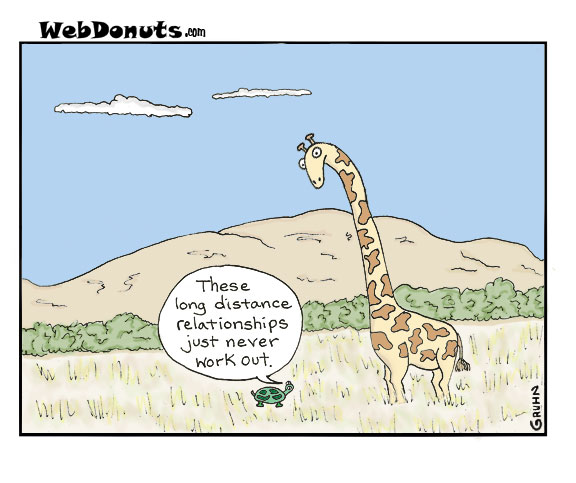
\includegraphics[height=6.5cm]{slides/distance.jpg}&
\vspace{-2.3in}
outline:
\begin{enumerate}
\item motivation
\item metric spaces
\item other data structures
\item simplified cover tree
\item nearest ancestor tree
\item experiments
\item open problems
\end{enumerate}
\end{tabular}
\end{frame}

%%%%%%%%%%%%%%%%%%%%%%%%%%%%%%%%%%%%%%%%

%\begin{frame}[fragile]{Why care about faster nearest neighbor queries?}
\begin{frame}[fragile]{Why care about cover trees?}
% image from: http://scikit-learn.org/0.11/auto_examples/neighbors/plot_classification.html

They speed up nearest neighbor queries, e.g. in
 $k$-nn classification:

\begin{center}
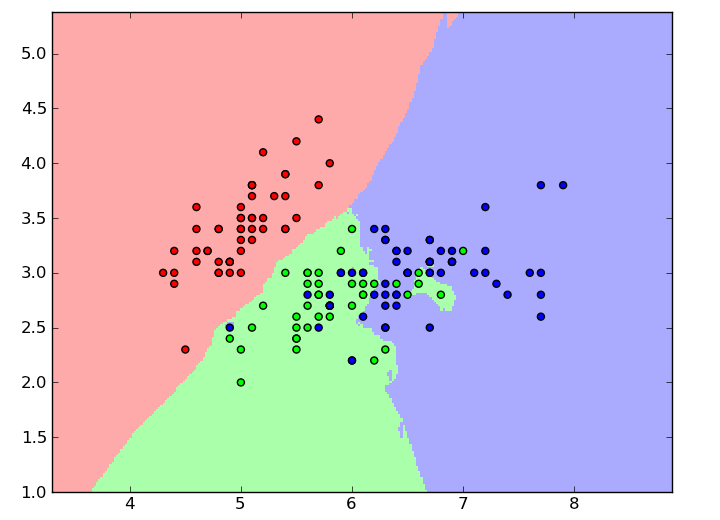
\includegraphics[width=5.5cm]{slides/knn.png}
\end{center}
%source: scikit learn

But neighbor queries are used in many other algorithms too:
\begin{itemize}
\item Localized support vector machines (Segata \& Blanzieri, 2010)
\item Dimensionality reduction (Lisitsyn \emph{et. al.}, 2013)
\item Reinforcement learning (Tziortziotis \emph{et. al.}, 2014)
\end{itemize}

\vspace{0.05in}
{\tiny image from: \url{http://scikit-learn.org}}

\end{frame}


\begin{frame}[fragile]{Nearest neighbor data structures for Euclidean distance}

%\begin{tikzpicture}
%\draw (-3,2) -- (9,2);
%%\draw (4,1.3) -- (8,1.3);
%\node at (0,0) {
    %\resizebox{6cm}{!}{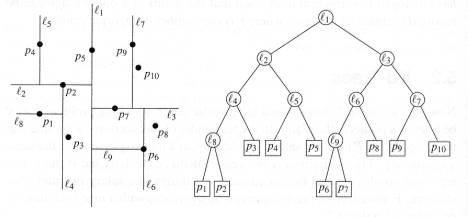
\includegraphics[width=12cm]{slides/kdtree.jpg}}
%};
%\node at (6,1.5) { \textbf{kd-tree} };
%\node at (6,0.5) { popular in machine learning libraries };
%\node at (6,-0.5) { MLPack, scikit, R, matlab, weka };
%
%\draw (-3,-2) -- (9,-2);
%%\draw (4,-2.7) -- (8,-2.7);
%\node at (0,-4) {
    %\resizebox{6cm}{!}{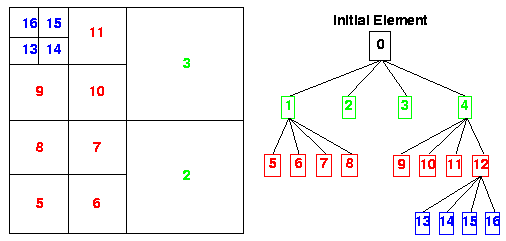
\includegraphics[width=12cm]{slides/quadtree.png}}
%};
%\node at (6,-2.5) { \textbf{quad/oct-tree} };
%%\node at (6,-3.5) { not popular in machine learning libraries };
%\node at (6,-3.5) { mostly used in graphics };
%\node at (6,-4.5) { very bad in high dimensions };
%\draw (-3,-6) -- (9,-6);
%\end{tikzpicture}

\begin{tabular}{m{6cm}m{5.2cm}}
\hline
& \\
%\vspace{0.1in}
\resizebox{6cm}{!}{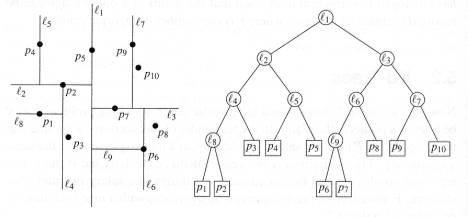
\includegraphics[width=12cm]{slides/kdtree.jpg}} &
%\begin{tabular}{c}
%\vspace{-0.5in}
%$k$d-tree \\
%\\
%popular in machine learning: \\
%\\
%MLPack, scikit, R, matlab, weka
%\end{tabular}
%\centering
\begin{center}
\textbf{kd-tree}

popular in machine learning

MLPack, scikit, R, matlab, weka

\vspace{0.15in}
(Friedman \emph{et al.}, 1977)
\end{center}
\\
\hline
&\\
%\hline
\vspace{0.0in}
\resizebox{6cm}{!}{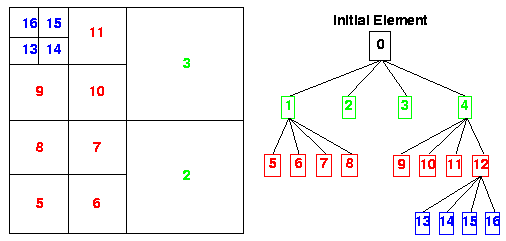
\includegraphics[width=12cm]{slides/quadtree.png}}
\vspace{-0.12in}
&
\begin{center}
\textbf{quad/oct-tree}

not popular in machine learning
\end{center}
%\\
%\hline
%$k$d-tree & quad/oct tree\\
%popular in machine learning & \\
%(MLPack, scikit learn, R, matlab, weka, etc.)
\\
\hline
\end{tabular}

\vspace{0.1in}
{\tiny
images from: \url{http://www.cs.sandia.gov/~kddevin/LB/figs}
}

%Friedman \emph{et al.}, Transactions on Mathematical Software, 1977
%
%(2234 citations)
%
%\vspace{0.25cm}
%simple, but only works on $\mathbb{R}^n$;
%
%\vspace{0.25cm}
%
%\vspace{0.25cm}
%
% image from: http://homes.ieu.edu.tr/hakcan/projects/kdtree/files/kdtree.jpg
\end{frame}




\begin{frame}[fragile]{Metric spaces generalize euclidean space}
\centering
\resizebox{!}{4.5cm}{
\begin{tikzpicture}[dot/.style={circle,inner sep=2pt,fill,name=#1},
    extended line/.style={shorten >=-#1,shorten <=-#1},
    extended line/.default=1cm]

% draw the grid
\uncover<1-3> {
    \draw[->] (0,-0.25) -- (0,5.25) ;
    \draw[->] (-0.25,0) -- (5.25,0) ;
    \foreach \i in {1,...,5} {
        \draw[dotted] (-0.25,\i) -- (5.25,\i);
        \draw[dotted] (\i,-0.25) -- (\i,5.25);
    }
}

% draw the points
\uncover<1-3> {
    \node [dot=a,label=above left:a] at (1,1) {};
    \node [dot=b,label=above:b] at (2,4) {};
    \node [dot=c,label=above right:c] at (4,2) {};
}

% draw the L2 metric
\uncover<1> {
    \draw (a) -- (b) -- (c) -- (a);
    \node at (3,1.25) {$\sqrt{10}$};
    \node at (1,2.75) {$\sqrt{10}$};
    \node at (3.5,3.25) {$2\sqrt{2}$};
    \node at (8, 4.5) {
        Euclidean distance:
        };
    \node at (9,2.5) {

        $\begin{aligned}
        \mathcal{X}& = \mathbb{R}^n \\
        \displaystyle
        d(x,y)
        &=
        \displaystyle
        \left(\sum_{i=1}^n (x_i-y_i)^2\right)^{\frac 1 2} \\
        \end{aligned}$
        };
    \node at (9, 0.5) { Runtime to calculate distance: $O(n)$ };
}

% draw the L1 metric
\uncover<2> {
    \draw (a) -- (1,4) -- (b) -- (4,4) -- (c) -- (4,1) -- (a);
    \node at (2.5,1.25) {$4$};
    \node at (1.25,2.75) {$4$};
    \node at (3.5,3.5) {$4$};
    \node at (9, 4.5) {
        $L_1$ (Manhattan, taxicab) distance:
        };
    \node at (9,2.5) {
        $\begin{aligned}
        \mathcal{X}& = \mathbb{R}^n \\
        \displaystyle
        d(x,y)
        &=
        \displaystyle
        \sum_{i=1}^n |x_i-y_i| \\
        \end{aligned}$
        };
    \node at (9, 0.5) { Runtime to calculate distance: $O(n)$ };
}

% draw the Linf metric
\uncover<3> {
    \draw (a) -- (1,4);
    \draw (4,4) -- (c);
    \draw (a) -- (4,1);
    \node at (2.5,1.25) {$3$};
    \node at (1.25,2.75) {$3$};
    \node at (3.5,3.5) {$2$};
    \node at (8, 4.5) {
        $L_\infty$ (sup) distance:
        };
    \node at (9,2.5) {
        $\begin{aligned}
        \mathcal{X}& = \mathbb{R}^n \\
        \displaystyle
        d(x,y)
        &=
        \displaystyle
        \sup_{i\in\{1..n\}} |x_i-y_i| \\
        \end{aligned}$
        };
    \node at (9, 0.5) { Runtime to calculate distance: $O(n)$ };
}

% draw the Lebesgue metric
%\uncover<4> {
    %\node at (9, 4.5) {
        %Lebesgue family of distances:
        %};
    %\node at (9,2.5) {
        %$\begin{aligned}
        %\mathcal{X}& = \mathbb{R}^n \\
        %\displaystyle
        %d(x,y)
        %&=
        %\displaystyle
        %\left(\sum_{i\in\{1..n\}} |x_i-y_i|^n\right)^{\frac 1 n} \\
        %\end{aligned}$
        %};
    %\node at (9, 0.5) { Runtime to calculate distance: $O(n)$ };
%}
%
%% graph distances
%\uncover <6-7> {
    %\draw[color=red,line width=2pt] (3.35,3.1) -- (3.65,3.4);
    %\node[color=red] at (4,3.25) {\textbf{1?}};
%}
%\uncover<6> {
    %\draw[color=red,line width=2pt] (6,0) -- (12,5);
%}
%
%\uncover<5-6> {
    %\draw (a) -- (b) -- (c) -- (a);
    %\node at (3,1.25) {$2$};
    %\node at (1,2.75) {$4$};
    %\node at (3.5,3.25) {$5$};
    %\node at (9, 4.5) {
        %weighted, fully-connected graph distance
        %};
    %\node at (9,2.5) {
        %$\begin{aligned}
        %\mathcal{X}& = \{a,b,c\} \\
        %\displaystyle
        %d(x,y)
        %&=
        %\text{edge weight}
        %\end{aligned}$
        %};
    %\node at (9, 0.5) { Runtime to calculate distance: $O(1)$ };
%}
%
%% graph distances
%\uncover<7> {
    %\draw (a) -- (b) -- (c) -- (a);
    %\node at (3,1.25) {$2$};
    %\node at (1,2.75) {$4$};
    %\node at (3.5,3.25) {$5$};
    %\node at (9, 4.5) {
        %Dijkstra graph distance
        %};
    %\node at (9,2.5) {
        %$\begin{aligned}
        %\mathcal{X}& = \{a,b,c\} \\
        %\displaystyle
        %d(x,y)
        %&=
        %\text{shortest path between $x$ and $y$}
        %\end{aligned}$
        %};
    %\node at (9, 0.5) { Runtime to calculate distance: $O(e+v\log v)$ };
%}
%
%% graph distances
%\uncover<8> {
    %\draw (a) -- (b);
    %\draw (c) -- (a);
    %\node at (3,1.25) {$2$};
    %\node at (1,2.75) {$4$};
    %\node at (9, 4.5) {
        %Dijkstra graph distance
        %};
    %\node at (9,2.5) {
        %$\begin{aligned}
        %\mathcal{X}& = \{a,b,c\} \\
        %\displaystyle
        %d(x,y)
        %&=
        %\text{shortest path between $x$ and $y$}
        %\end{aligned}$
        %};
    %\node at (9, 0.5) { Runtime to calculate distance: $O(e+v\log v)$ };
%}
%
%% graph distances
%\uncover<9> {
    %\draw (a) -- (b);
    %\node at (1,2.75) {$4$};
    %\node at (9, 4.5) {
        %Dijkstra graph distance
        %};
    %\node at (9,2.5) {
        %$\begin{aligned}
        %\mathcal{X}& = \{a,b,c\} \\
        %\displaystyle
        %d(x,y)
        %&=
        %\text{shortest path between $x$ and $y$}
        %\end{aligned}$
        %};
    %\node at (9, 0.5) { Runtime to calculate distance: $O(e+v\log v)$ };
%}
%
%% graph distances
%\uncover<10> {
    %\node at (8, 4.5) {
        %trivial distance
        %};
    %\node at (9,2.5) {
        %$\begin{aligned}
        %\mathcal{X}& = \{a,b,c\} \\
        %\displaystyle
        %d(x,y)
        %&=
        %\infty
        %\end{aligned}$
        %};
    %\node at (9, 0.5) { Runtime to calculate distance: $O(1)$ };
%}

% graph distances
\uncover<4> {
    \node at (1,3) {
        $d \left(
        \text{
        \begin{tikzpicture}
        \node at (0,2) {};
        \node [dot= ] at (1,1) {};
        \node [dot= ] at (1,0) {};
        \node [dot= ] at (0,1) {};
        \draw (1,1) -- (1,0) -- (0,1) -- (1,1);
        \end{tikzpicture}
        ,
        \begin{tikzpicture}
        \node at (0,2) {};
        \node [dot= ] at (1,1) {};
        \node [dot= ] at (1,0) {};
        \node [dot= ] at (0,1) {};
        \node [dot= ] at (0,0) {};
        \draw (1,1) -- (1,0) -- (0,1) -- (1,1) -- (0,0) -- (0,1) -- (1,0) -- (0,0);
        \end{tikzpicture}
        }
        \right)$
    };
    \node at (9, 4.5) {
        \emph{graph metrics} are distances between graphs
        };
    \node at (9,2.5) {
        $\begin{aligned}
        \mathcal{X}& = \text{set of all graphs} \\
        \displaystyle
        d(x,y)
        &=
        \text{many possibilities}
        \end{aligned}$
        };
    \node at (9, 0.5) { Runtime to calculate distance: varies };
}

\end{tikzpicture}
}
\begin{defn}
A \emph{metric space} is a set $\mathcal{X}$ equiped with a distance function $d : \mathcal{X} \times \mathcal{X} \rightarrow \mathbb{R}$ such that:
\begin{center}
\begin{tabular}{ll}
$d(x,y) \ge 0$ & $d(x,y) = 0$ iff $x=y$ \\
$d(x,y) = d(y,x)$ & $d(x,z) \le d(x,y) + d(y,z)$ \\
\end{tabular}
\end{center}
\end{defn}
\end{frame}


\begin{frame}[fragile]{Metrics for proteins}

\vspace{-0.3in}
\begin{center}
\begin{tikzpicture}
\node at (0,0) {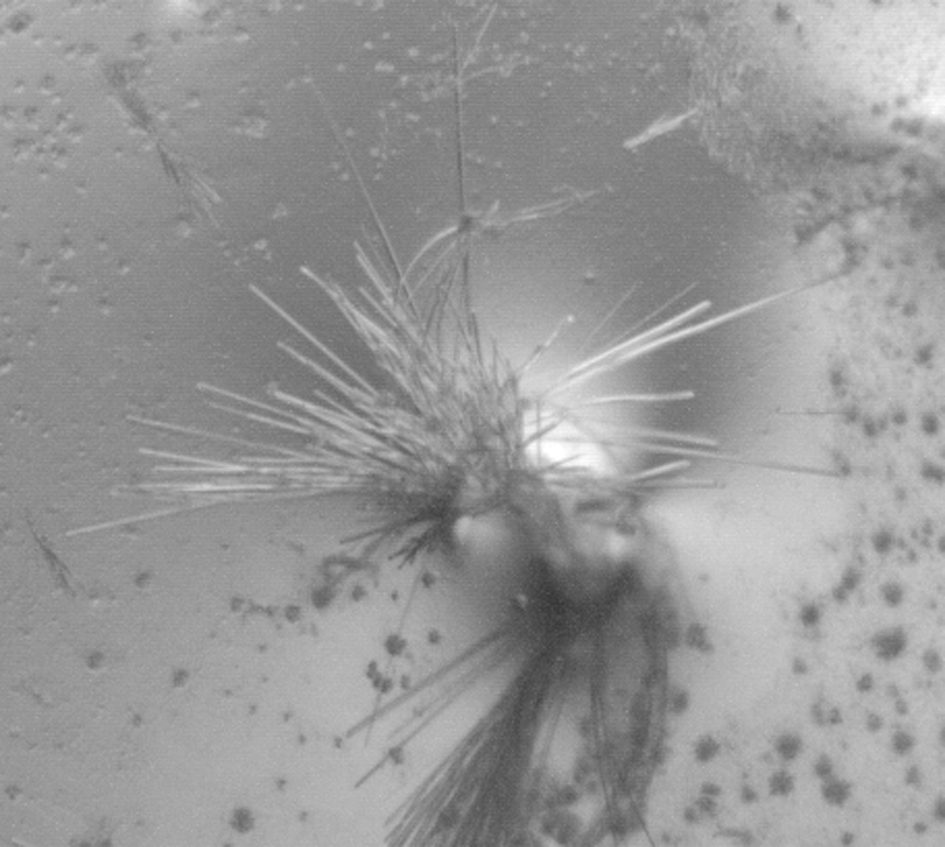
\includegraphics[width=4cm]{slides/xrayprotein}};
\node at (6,0) {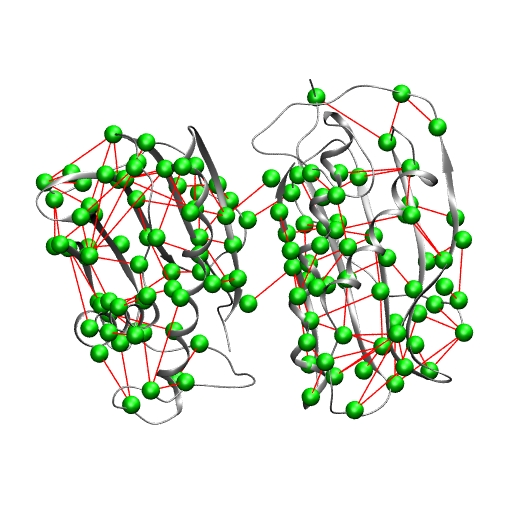
\includegraphics[width=4cm]{slides/ProteinGraphs}};

\draw[->,line width=4pt] (2.75,0) -- (3.75,0);
\end{tikzpicture}
\end{center}

\vspace{-0.2in}

%The protein databank contains information on $\sim$100,000 proteins
%
%\vspace{0.1in}
Protein structure (and hence function) can be modeled as a graph

\vspace{0.1in}
The random walk graph kernel is a commonly used protein metric

\vspace{0.1in}
This is an \emph{expensive} metric, taking time $O(v^3)$

\vspace{0.1in}
(Vishwanathan \emph{et. al.}, 2010)

\vspace{0.15in}
{\tiny
images from: \url{http://www.lunenfeld.ca}, and \url{http://vishgraph.mbu.iisc.ernet.in/GraProStr/}
}

\end{frame}



\begin{frame}[fragile]{Metrics for images}
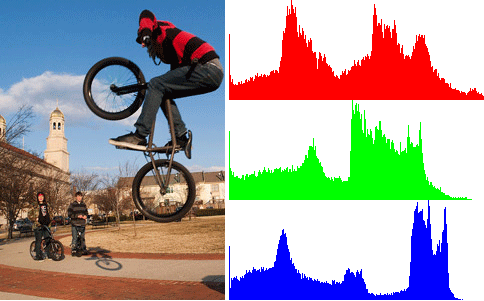
\includegraphics[width=6cm]{slides/imagehistogram2.png}
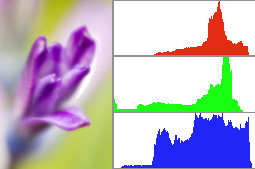
\includegraphics[width=6cm]{slides/imagehistogram3b.jpg}

\vspace{0.15in}
There are \emph{lots} of distance metrics for images.
Histogram metrics follow the two step process:
\begin{itemize}
\item generate histograms (usually of colors)
\item define a distance between histograms
\end{itemize}

Earth mover's distance is a popular but slow metric.
It runs in time $O(b^3 \log b)$, where $b$ is the size of the histogram.
(Rubner \emph{et. al.}, 1998)

\vspace{0.05in}
{\tiny
images from: \url{http://billmill.org/the_histogram.html}
}
\end{frame}


%\begin{frame}[fragile]{metrics for images}
%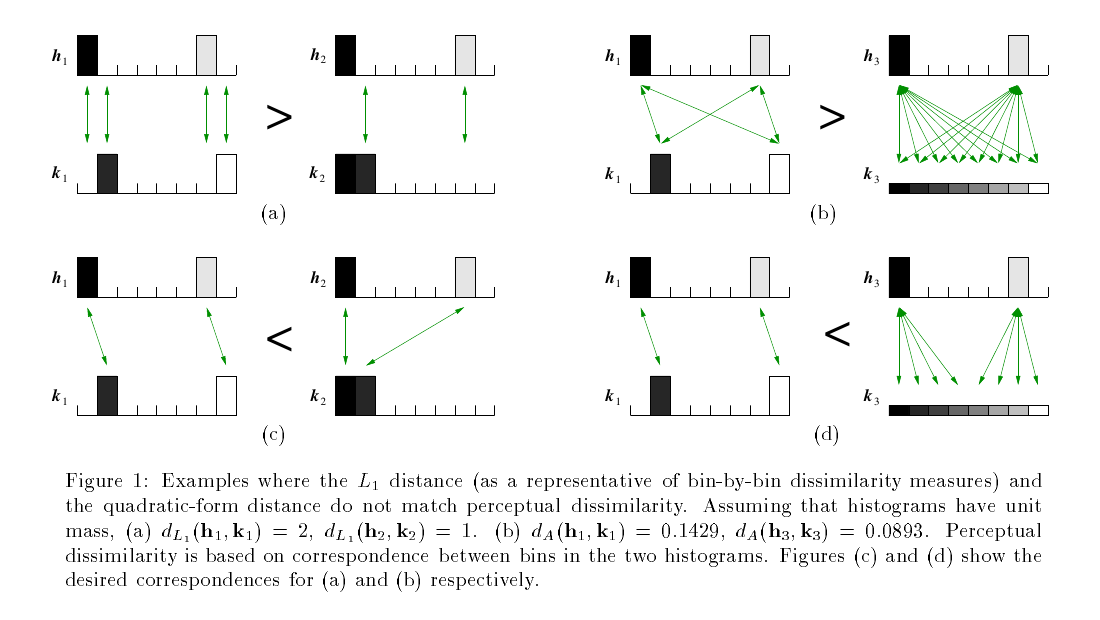
\includegraphics[width=12cm]{slides/emd.png}
%
%\end{frame}

\begin{frame}[fragile]{Metrics can be learned}
\begin{align*}
%\phi & : \set X \to \set X ~~~~~ \text{learned from data}\\
d'_\phi(x,y) & = d(\phi(x),\phi(y))\\
\phi &= \argmin_{\phi} \sum_{(x,y) \in \set X \times \set X} \ell(x,y;\phi)
\end{align*}
%% image from: http://upload.wikimedia.org/wikipedia/commons/f/fd/Lle_hlle_swissroll.png
%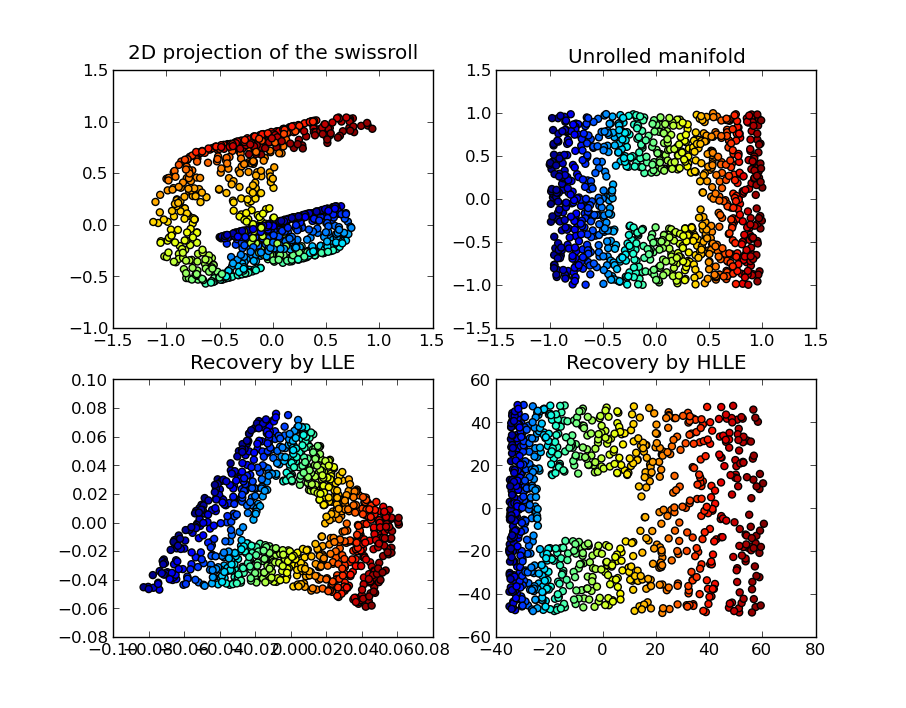
\includegraphics[height=9cm,width=12cm]{slides/swissroll.png}
% http://scikit-learn.org/0.12/_images/plot_compare_methods_11.png
\hspace{-1.5cm}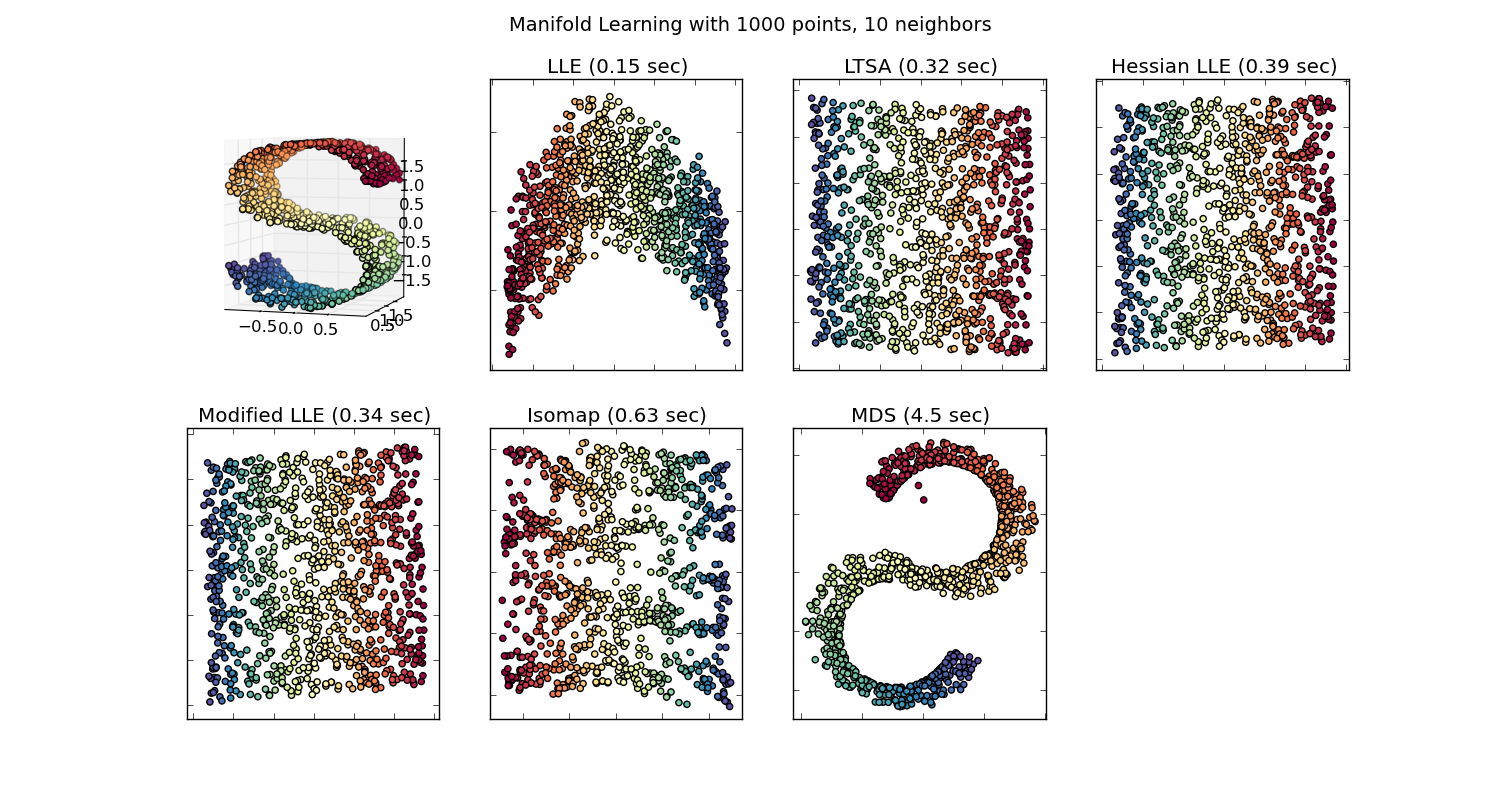
\includegraphics[height=6cm,width=15cm]{slides/manifold.png}
\end{frame}



\begin{frame}[fragile]{Nearest neighbor data structures for arbitrary metric spaces}

%\begin{tikzpicture}
%\node at (0,2) {
    %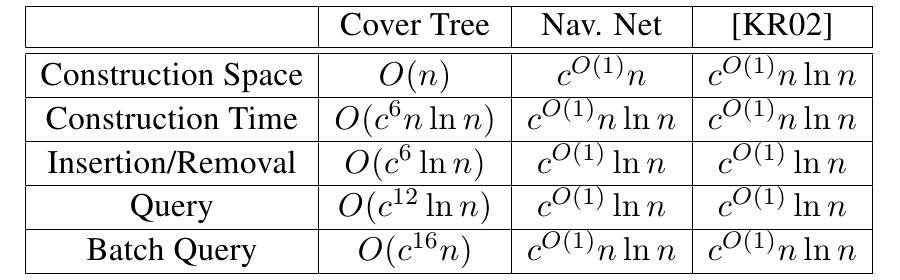
\includegraphics[width=12cm]{covertree/runtimes}


{\footnotesize
    \begin{tabular}{>\centering m{2cm}|>\centering m{2.0cm}|>\centering m{2.0cm}|>\centering m{2.0cm}|c}
    \hline
    & \footnotesize Cover Tree
    & \footnotesize Nav. Net
    & \footnotesize Met. Skip List
    & \footnotesize Ball Tree
    \\
    \hline
    \hline
    Construction space & $O(n)$ & $c^{O(1)}n$ & $c^{O(1)}n \log n$ & $O(n)$ \\
    Construction time & $O(c^6 n\log n)$ & $c^{O(1)}n\log n$ & $c^{O(1)}n \log n$ & $O(n^2)$ \\
    Insertion time (1 pt) & $O(c^6 \log n)$ & $c^{O(1)}\log n$ & $c^{O(1)} \log n$ & $O(n)$ \\
    Query time ~~~(1 pt) & $O(c^{12} \log n)$ & $c^{O(1)}\log n$ & $c^{O(1)} \log n$ &  $O(n)$\\
    Query time ~~~(n pts) & $O(c^{16} n)$ & $c^{O(1)}n\log n$ & $c^{O(1)}n \log n$ &  $O(n^2)$\\
    \hline
    & \footnotesize Beygelzimer ~~~\emph{et. al.}, 2006
    & \footnotesize Krauthgamer and Lee, 2004
    & \footnotesize Karger and Ruhl, 2002
    & \begin{tabular}{c}
        Omohundro,\\
        1989
      \end{tabular}
    \\
    \hline

    \end{tabular}
}
%};

\vspace{0.05in}
The variable $c$ is a measure of dimension (defined on next slide).

%\footnotesize
%\node at (-1,-0.4) { (Beygelzimer \emph{et. al.}, 2006)};
%\node at (2,-1) { (Krauthgamer and Lee, 2004)};
%\node at (4,-0.4) { (Karger and Ruhl, 2002) };
%\draw[->] (-1,-0.25) -- (-0.9,0.1);
%\draw[->] (1.3,-0.75) -- (1.5,0.1);
%\end{tikzpicture}

%Karger and Ruhl, Symposium on the Theory of Computing, 2002
%
%\vspace{0.15in}
%Krauthgamer and Lee, Symposium on Discrete Algorithms, 2004
%
%\vspace{0.15in}
%Beygelzimer, Kakade, and Langford, ICML, 2006

\vspace{0.05in}
Recent research either:
\begin{itemize}
\item Extends the analysis on cover trees {\footnotesize (Ram \emph{et. al.}, 2010; Curtin \emph{et. al.}, 2013)}
\item Focuses on \emph{approximate} queries (too many papers to list)
\end{itemize}

%\vspace{0.15in}
%More recent research focuses on \emph{approximate} queries: LHS, Spill trees
%\textbf{open problem}: construct a data structure in time $O(c^{O(1)}n)$ for some dimensionality $c$; is it even possible?
%\vspace{0.15in}

\end{frame}


%\begin{frame}[fragile]{The expansion constant $c$}
%
%Given a metric space $X$ with distance $d : X \times X \to \mathbb{R}$, define
%\vspace{0.15in}
%
%\textbf{ball of radius $r$ centered at point $p$ }:
%$$
%B(p,r) = \{q \in X : d(p,q) \le r \}
%$$
%
%%\textbf{expansion constant $(c)$}: the smallest value $c \ge 2$ such that
%%$$
%%|B(p,2r)| \le c|B(p,r)|
%%$$
%%for every $p$ in the metric space $X$ and $r\ge0$.
%
%\textbf{expansion constant}:
%$$
%c = \sup_{p\in X, r\ge0} \left\{
    %\frac{|B(p,2r)|}{|B(p,r)|}
      %\right\}
%$$
%
%\hrule
%
%\vspace{0.15in}
%properties of the expansion constant:
%\begin{enumerate}
%\item dimension $(=\log c)$ of $\mathbb{R}^n$ is $O(n)$
%\item roughly captures the ``intrinsic dimensionality'' of $X$
%\item adding a single new point to $X$ can increase $c$ by an arbitrary amount;
%
%there are subsets of $\mathbb{R}^2$ with $c=\infty$
%\end{enumerate}
%
%\end{frame}

%%%%%%%%%%%%%%%%%%%%%%%%%%%%%%%%%%%%%%%%%%%%%%%%%%%%%%%%%%%%%%%%%%%%%%%%%%%%%%%%

\begin{frame}[fragile]{The expansion constant $c$ is a type of dimension}

The \textbf{expansion constant} is defined as:
$$
c = \sup_{p\in X, r\ge0} \left\{
    \frac{|B(p,2r)|}{|B(p,r)|}
      \right\}
$$
where
$$
B(p,r) = \{q \in X : d(p,q) \le r \}
$$
is the ball of radius $r$ centered at point $p$.
\vspace{0.15in}

\hrule
\vspace{0.15in}

\begin{tabular}{m{4cm}m{7cm} }
\resizebox{!}{3.5cm}{
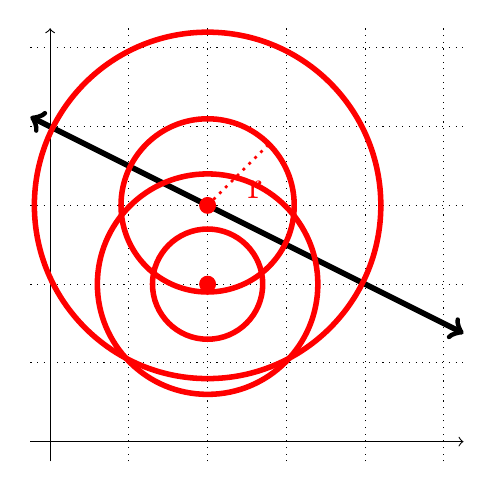
\begin{tikzpicture}[dot/.style={circle,inner sep=2pt,fill,name=#1},
    extended line/.style={shorten >=-#1,shorten <=-#1},
    extended line/.default=1cm]

% draw the grid
\draw[->] (0,-0.25) -- (0,5.25) ;
\draw[->] (-0.25,0) -- (5.25,0) ;
\foreach \i in {1,...,5} {
    \draw[dotted] (-0.25,\i) -- (5.25,\i);
    \draw[dotted] (\i,-0.25) -- (\i,5.25);
}

\uncover<2-3> {
    \draw[line width=2pt,<->] (-0.25,4.125) -- (5.25,1.375);
}

\uncover<1-2> {
    \node at (2.6,3.2) { \textcolor{red}{\Large r} };
    \path[draw=red,dotted,line width=1pt] (2,3) -- (2.8,3.8);
    \path[draw=red,fill=red] (2,3) circle (0.1);
    \path[draw=red,line width=2pt] (2,3) circle (1.1);
    \path[draw=red,line width=2pt] (2,3) circle (2.2);
}

\uncover<3> {
    %\node at (2.6,3.2) { \textcolor{red}{\Large r} };
    %\path[draw=red,dotted,line width=1pt] (2,2) -- (2.8,3.8);
    \path[draw=red,fill=red] (2,2) circle (0.1);
    \path[draw=red,line width=2pt] (2,2) circle (0.7);
    \path[draw=red,line width=2pt] (2,2) circle (1.4);
}

%\node[text width=8cm, align=left] at (10,3.5) {
    %\Large
%
%
    %%with the Euclidean distance.
%};


\end{tikzpicture}
}
&
\uncover<1> {
    \textbf{Example 1:}
    In the metric space $\mathbb{R}^2$,
    $$
    c
    = \frac{\pi(2r)^2}{\pi r^2}
    = 4
    $$
    Define the \textbf{expansion dimension} as $\log_2 c$.
    Then the expansion dimension of $\mathbb{R}^n$ is $n$.
    %In general, the dimension of $\mathbb{R}^n$ is $O(n)$.
}
\\ &
\vspace{-1.5in}
\uncover<2> {
    \textbf{Example 2:}
    In the subspace of $\mathbb{R}^2$ given by
    $$
    %\mathcal{X} = \{ (x,y) : y = -0.5x+4 \}
    \{ (x,y) : y = -0.5x+4 \}
    $$
    we have
    $$
    c
    = \frac{2r}{ r}
    = 2
    $$
    %So the dimensionality $\log_2 c = 1$.
}
\\ &
\vspace{-1.75in}
\uncover<3> {
    \textbf{Example 3:}
    In the subspace of $\mathbb{R}^2$ given by
    $$
    %\mathcal{X} = \{ (x,y) : y = -0.5x+4 \}
    \{ (x,y) : y = -0.5x+4 \} \cup \{(2,2)\}
    $$
    we have
    $
    c
    %= \frac{\infty}{0}
    = \infty
    $
    %so the expansion dimension is also $\infty$.
}


\end{tabular}

\end{frame}


\begin{frame}[fragile]{The simplified cover tree}

\begin{center}
\begin{tikzpicture}
    [ draw
    , every node/.style={minimum size=10mm,fill=white}
    , level/.style={sibling distance = 23mm/#1, level distance=12mm}
    %,    level distance = 1.5cm}
    , sibling distance=8mm
    ]
\draw (-2.3,0) -- (8.6,0)[dotted];
\draw (-2.3,-12mm) -- (8.6,-12mm)[dotted];
\draw (-2.3,-24mm) -- (8.6,-24mm)[dotted];
\node[shape=circle,draw] at (2.5,0) {10}
    child { node[circle,draw] {8}
        child { node[circle,draw] {7}  }
        child { node[circle,draw] {9} }
        }
    child { node[circle,draw] {12}
        %child { node[circle,draw,fill=lightred,line width=1pt] {9}  }
        %child { node[circle,draw] {13} }
        }
    ;
%\node[shape=circle,draw] at (5,0) {10}
    %child { node[circle,draw] {8}
        %child { node[circle,draw] {7}  }
        %child { node[circle,draw,fill=lightgreen,line width=1pt] {9} }
        %}
    %child { node[circle,draw] {12}
        %child { node[circle,draw,fill=lightgreen,line width=1pt] {11}  }
        %child { node[circle,draw] {13} }
        %}
    %;
\node[fill=none] at (8,3mm) {level 3};
\node[fill=none] at (8,-9mm) {level 2};
\node[fill=none] at (8,-21mm) {level 1};
\end{tikzpicture}
\end{center}

\uncover<1> {
%\vspace{0.15in}
\textbf{The covering invariant.}
For every node $p$, define the function $\covdist p = \exprad p^{\level p}$.
For each child $q$ of $p$
$$
\dist p q \le \covdist p
$$

\vspace{0.15in}
\textbf{The separating invariant.}
For every node $p$, define the function $\sepdist p = \exprad p^{\level p-1}$.
For all distinct children $q_1$ and $q_2$ of $p$
$$
\dist{q_1}{q_2} \ge \sepdist p
$$
}

\uncover<2> {
\vspace{-1.70in}
Advantages of the simplified cover tree:
\vspace{0.05in}
\begin{itemize}
\item Maintains all runtime guarantees of the original cover tree.
\vspace{0.05in}

\item Significantly easier to understand and implement.

%\vspace{0.05in}
The original cover tree was described in terms of an infinitely large tree, only a subset of which actually gets implemented.

\vspace{0.05in}
\item Requires exactly $n$ nodes instead of $O(n)$ nodes.

%\vspace{0.05in}
Fewer nodes means a faster constant factor for all algorithms. %insertions and queries are faster.
\end{itemize}
\vspace{1.3in}
}

\end{frame}


\begin{frame}[fragile]{The simplified cover tree}

\centering
\graphicspath{{slides/paperimg/}}
% GNUPLOT: LaTeX picture with Postscript
\begingroup
  \makeatletter
  \providecommand\color[2][]{%
    \GenericError{(gnuplot) \space\space\space\@spaces}{%
      Package color not loaded in conjunction with
      terminal option `colourtext'%
    }{See the gnuplot documentation for explanation.%
    }{Either use 'blacktext' in gnuplot or load the package
      color.sty in LaTeX.}%
    \renewcommand\color[2][]{}%
  }%
  \providecommand\includegraphics[2][]{%
    \GenericError{(gnuplot) \space\space\space\@spaces}{%
      Package graphicx or graphics not loaded%
    }{See the gnuplot documentation for explanation.%
    }{The gnuplot epslatex terminal needs graphicx.sty or graphics.sty.}%
    \renewcommand\includegraphics[2][]{}%
  }%
  \providecommand\rotatebox[2]{#2}%
  \@ifundefined{ifGPcolor}{%
    \newif\ifGPcolor
    \GPcolortrue
  }{}%
  \@ifundefined{ifGPblacktext}{%
    \newif\ifGPblacktext
    \GPblacktextfalse
  }{}%
  % define a \g@addto@macro without @ in the name:
  \let\gplgaddtomacro\g@addto@macro
  % define empty templates for all commands taking text:
  \gdef\gplbacktext{}%
  \gdef\gplfronttext{}%
  \makeatother
  \ifGPblacktext
    % no textcolor at all
    \def\colorrgb#1{}%
    \def\colorgray#1{}%
  \else
    % gray or color?
    \ifGPcolor
      \def\colorrgb#1{\color[rgb]{#1}}%
      \def\colorgray#1{\color[gray]{#1}}%
      \expandafter\def\csname LTw\endcsname{\color{white}}%
      \expandafter\def\csname LTb\endcsname{\color{black}}%
      \expandafter\def\csname LTa\endcsname{\color{black}}%
      \expandafter\def\csname LT0\endcsname{\color[rgb]{1,0,0}}%
      \expandafter\def\csname LT1\endcsname{\color[rgb]{0,1,0}}%
      \expandafter\def\csname LT2\endcsname{\color[rgb]{0,0,1}}%
      \expandafter\def\csname LT3\endcsname{\color[rgb]{1,0,1}}%
      \expandafter\def\csname LT4\endcsname{\color[rgb]{0,1,1}}%
      \expandafter\def\csname LT5\endcsname{\color[rgb]{1,1,0}}%
      \expandafter\def\csname LT6\endcsname{\color[rgb]{0,0,0}}%
      \expandafter\def\csname LT7\endcsname{\color[rgb]{1,0.3,0}}%
      \expandafter\def\csname LT8\endcsname{\color[rgb]{0.5,0.5,0.5}}%
    \else
      % gray
      \def\colorrgb#1{\color{black}}%
      \def\colorgray#1{\color[gray]{#1}}%
      \expandafter\def\csname LTw\endcsname{\color{white}}%
      \expandafter\def\csname LTb\endcsname{\color{black}}%
      \expandafter\def\csname LTa\endcsname{\color{black}}%
      \expandafter\def\csname LT0\endcsname{\color{black}}%
      \expandafter\def\csname LT1\endcsname{\color{black}}%
      \expandafter\def\csname LT2\endcsname{\color{black}}%
      \expandafter\def\csname LT3\endcsname{\color{black}}%
      \expandafter\def\csname LT4\endcsname{\color{black}}%
      \expandafter\def\csname LT5\endcsname{\color{black}}%
      \expandafter\def\csname LT6\endcsname{\color{black}}%
      \expandafter\def\csname LT7\endcsname{\color{black}}%
      \expandafter\def\csname LT8\endcsname{\color{black}}%
    \fi
  \fi
  \setlength{\unitlength}{0.0500bp}%
  \begin{picture}(5040.00,3772.00)%
    \gplgaddtomacro\gplbacktext{%
      \csname LTb\endcsname%
      \put(1166,780){\makebox(0,0)[r]{\strut{} 0}}%
      \put(1166,1053){\makebox(0,0)[r]{\strut{} 0.1}}%
      \put(1166,1325){\makebox(0,0)[r]{\strut{} 0.2}}%
      \put(1166,1598){\makebox(0,0)[r]{\strut{} 0.3}}%
      \put(1166,1871){\makebox(0,0)[r]{\strut{} 0.4}}%
      \put(1166,2144){\makebox(0,0)[r]{\strut{} 0.5}}%
      \put(1166,2416){\makebox(0,0)[r]{\strut{} 0.6}}%
      \put(1166,2689){\makebox(0,0)[r]{\strut{} 0.7}}%
      \put(1166,2962){\makebox(0,0)[r]{\strut{} 0.8}}%
      \put(1166,3234){\makebox(0,0)[r]{\strut{} 0.9}}%
      \put(1166,3507){\makebox(0,0)[r]{\strut{} 1}}%
      \put(1661,648){\rotatebox{-45}{\makebox(0,0)[l]{\strut{}yearpredict}}}%
      \put(2023,648){\rotatebox{-45}{\makebox(0,0)[l]{\strut{}twitter}}}%
      \put(2386,648){\rotatebox{-45}{\makebox(0,0)[l]{\strut{}tinyImages}}}%
      \put(2748,648){\rotatebox{-45}{\makebox(0,0)[l]{\strut{}mnist}}}%
      \put(3111,648){\rotatebox{-45}{\makebox(0,0)[l]{\strut{}corel}}}%
      \put(3473,648){\rotatebox{-45}{\makebox(0,0)[l]{\strut{}covtype}}}%
      \put(3836,648){\rotatebox{-45}{\makebox(0,0)[l]{\strut{}artificial40}}}%
      \put(4198,648){\rotatebox{-45}{\makebox(0,0)[l]{\strut{}faces}}}%
      \put(176,2143){\rotatebox{-270}{\makebox(0,0){\strut{}fraction of nodes in the original cover tree }}}%
      \put(396,2143){\rotatebox{-270}{\makebox(0,0){\strut{} required for the simplified cover tree}}}%
    }%
    \gplgaddtomacro\gplfronttext{%
    }%
    \gplbacktext
    \put(0,0){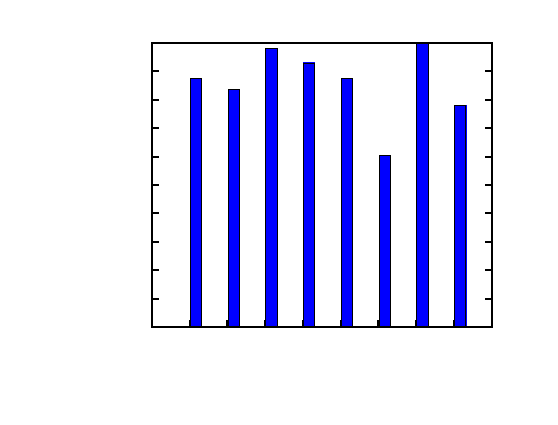
\includegraphics{nodes}}%
    \gplfronttext
  \end{picture}%
\endgroup


\end{frame}

\begin{frame}[fragile]{The nearest ancestor cover tree}

\definecolor{lightred}{rgb}{1,0.8,0.8}
\definecolor{lightgreen}{rgb}{0.8,1,0.8}
\begin{center}
\begin{tikzpicture}
    [ draw
    , every node/.style={minimum size=10mm,fill=white}
    , level/.style={sibling distance = 23mm/#1, level distance=12mm}
    %,    level distance = 1.5cm}
    , sibling distance=8mm
    ]
\draw (-2.3,0) -- (8.6,0)[dotted];
\draw (-2.3,-12mm) -- (8.6,-12mm)[dotted];
\draw (-2.3,-24mm) -- (8.6,-24mm)[dotted];
\node[shape=circle,draw] at (0,0) {10}
    child { node[circle,draw] {8}
        child { node[circle,draw] {7}  }
        child { node[circle,draw,fill=lightred,line width=1pt] {11} }
        }
    child { node[circle,draw] {12}
        child { node[circle,draw,fill=lightred,line width=1pt] {9}  }
        child { node[circle,draw] {13} }
        }
    ;
\node[shape=circle,draw] at (5,0) {10}
    child { node[circle,draw] {8}
        child { node[circle,draw] {7}  }
        child { node[circle,draw,fill=lightgreen,line width=1pt] {9} }
        }
    child { node[circle,draw] {12}
        child { node[circle,draw,fill=lightgreen,line width=1pt] {11}  }
        child { node[circle,draw] {13} }
        }
    ;
\node[fill=none] at (8,3mm) {level 3};
\node[fill=none] at (8,-9mm) {level 2};
\node[fill=none] at (8,-21mm) {level 1};
\end{tikzpicture}
\end{center}

A \textbf{nearest ancestor cover tree} is a simplified cover tree where every point $p$ satisfies the additional invariant that if $q_1$ is an ancestor of $p$ and $q_2$ is a sibling of $q_1$, then
$$
d(p,q_1) \le d(p,q_2)
$$

\end{frame}

%%%%%%%%%%%%%%%%%%%%%%%%%%%%%%%%%%%%%%%%%%%%%%%%%%%%%%%%%%%%%%%%%%%%%%%%%%%%%%%%

\begin{frame}[fragile]{Inserting into a nearest ancestor cover tree}
Inserting into a nearest ancestor cover tree can require rebalancing.
\begin{center}
\begin{tikzpicture}
    [ draw
    , every node/.style={minimum size=10mm,fill=white}
    , level/.style={sibling distance = 23mm/#1, level distance=12mm}
    %,    level distance = 1.5cm}
    , sibling distance=8mm
    ]
\draw (-2.3,0) -- (8.6,0)[dotted];
\draw (-2.3,-12mm) -- (8.6,-12mm)[dotted];
\draw (-2.3,-24mm) -- (8.6,-24mm)[dotted];

\uncover<1> {
\node[shape=circle,draw] at (2.5,0) {10}
    child { node[circle,draw] {8}
        child [color=white] {}
        child { node[circle,draw] {11} }
        }
    child [ color=white ] { %node[circle,draw] {12}
        %child { node[circle,draw,fill=lightred,line width=1pt] {9}  }
        %child { node[circle,draw] {13} }
        }
    ;
}

\uncover<2> {
\node[shape=circle,draw] at (2.5,0) {10}
    child { node[circle,draw] {8}
        child [color=white] {}
        child { node[circle,fill=lightred,draw] {11} }
        }
    child  { node[circle,draw] {12}
        %child { node[circle,draw,fill=lightred,line width=1pt] {9}  }
        %child { node[circle,draw] {13} }
        }
    ;
}

\uncover<3> {
\node[shape=circle,draw] at (2.5,0) {10}
    child { node[circle,draw] {8}
        child [color=white] {}
        child [color=white] {}
        }
    child  { node[circle,draw] {12}
        child { node[circle,fill=lightgreen,draw] {11} }
        child [color=white] {}
        %child { node[circle,draw,fill=lightred,line width=1pt] {9}  }
        %child { node[circle,draw] {13} }
        }
    ;
}
\node[fill=none] at (8,3mm) {level 3};
\node[fill=none] at (8,-9mm) {level 2};
\node[fill=none] at (8,-21mm) {level 1};
\end{tikzpicture}
\end{center}

\vspace{0.15in}
No runtime bounds on the rebalancing step.

\vspace{0.15in}
In practice, queries are faster but construction is slower.
\end{frame}

%%%%%%%%%%%%%%%%%%%%%%%%%%%%%%%%%%%%%%%%%%%%%%%%%%%%%%%%%%%%%%%%%%%%%%%%%%%%%%%%

\begin{frame}[fragile]{Comparing cover trees on \emph{construction} time}
\centering
\graphicspath{{slides/paperimg/}}
% GNUPLOT: LaTeX picture with Postscript
\begingroup
  \makeatletter
  \providecommand\color[2][]{%
    \GenericError{(gnuplot) \space\space\space\@spaces}{%
      Package color not loaded in conjunction with
      terminal option `colourtext'%
    }{See the gnuplot documentation for explanation.%
    }{Either use 'blacktext' in gnuplot or load the package
      color.sty in LaTeX.}%
    \renewcommand\color[2][]{}%
  }%
  \providecommand\includegraphics[2][]{%
    \GenericError{(gnuplot) \space\space\space\@spaces}{%
      Package graphicx or graphics not loaded%
    }{See the gnuplot documentation for explanation.%
    }{The gnuplot epslatex terminal needs graphicx.sty or graphics.sty.}%
    \renewcommand\includegraphics[2][]{}%
  }%
  \providecommand\rotatebox[2]{#2}%
  \@ifundefined{ifGPcolor}{%
    \newif\ifGPcolor
    \GPcolortrue
  }{}%
  \@ifundefined{ifGPblacktext}{%
    \newif\ifGPblacktext
    \GPblacktextfalse
  }{}%
  % define a \g@addto@macro without @ in the name:
  \let\gplgaddtomacro\g@addto@macro
  % define empty templates for all commands taking text:
  \gdef\gplbacktext{}%
  \gdef\gplfronttext{}%
  \makeatother
  \ifGPblacktext
    % no textcolor at all
    \def\colorrgb#1{}%
    \def\colorgray#1{}%
  \else
    % gray or color?
    \ifGPcolor
      \def\colorrgb#1{\color[rgb]{#1}}%
      \def\colorgray#1{\color[gray]{#1}}%
      \expandafter\def\csname LTw\endcsname{\color{white}}%
      \expandafter\def\csname LTb\endcsname{\color{black}}%
      \expandafter\def\csname LTa\endcsname{\color{black}}%
      \expandafter\def\csname LT0\endcsname{\color[rgb]{1,0,0}}%
      \expandafter\def\csname LT1\endcsname{\color[rgb]{0,1,0}}%
      \expandafter\def\csname LT2\endcsname{\color[rgb]{0,0,1}}%
      \expandafter\def\csname LT3\endcsname{\color[rgb]{1,0,1}}%
      \expandafter\def\csname LT4\endcsname{\color[rgb]{0,1,1}}%
      \expandafter\def\csname LT5\endcsname{\color[rgb]{1,1,0}}%
      \expandafter\def\csname LT6\endcsname{\color[rgb]{0,0,0}}%
      \expandafter\def\csname LT7\endcsname{\color[rgb]{1,0.3,0}}%
      \expandafter\def\csname LT8\endcsname{\color[rgb]{0.5,0.5,0.5}}%
    \else
      % gray
      \def\colorrgb#1{\color{black}}%
      \def\colorgray#1{\color[gray]{#1}}%
      \expandafter\def\csname LTw\endcsname{\color{white}}%
      \expandafter\def\csname LTb\endcsname{\color{black}}%
      \expandafter\def\csname LTa\endcsname{\color{black}}%
      \expandafter\def\csname LT0\endcsname{\color{black}}%
      \expandafter\def\csname LT1\endcsname{\color{black}}%
      \expandafter\def\csname LT2\endcsname{\color{black}}%
      \expandafter\def\csname LT3\endcsname{\color{black}}%
      \expandafter\def\csname LT4\endcsname{\color{black}}%
      \expandafter\def\csname LT5\endcsname{\color{black}}%
      \expandafter\def\csname LT6\endcsname{\color{black}}%
      \expandafter\def\csname LT7\endcsname{\color{black}}%
      \expandafter\def\csname LT8\endcsname{\color{black}}%
    \fi
  \fi
  \setlength{\unitlength}{0.0500bp}%
  \begin{picture}(5040.00,3772.00)%
    \gplgaddtomacro\gplbacktext{%
      \csname LTb\endcsname%
      \put(1122,780){\makebox(0,0)[r]{\strut{} 0}}%
      \put(1122,1235){\makebox(0,0)[r]{\strut{} 1}}%
      \put(1122,1689){\makebox(0,0)[r]{\strut{} 2}}%
      \put(1122,2144){\makebox(0,0)[r]{\strut{} 3}}%
      \put(1122,2598){\makebox(0,0)[r]{\strut{} 4}}%
      \put(1122,3053){\makebox(0,0)[r]{\strut{} 5}}%
      \put(1622,648){\rotatebox{-45}{\makebox(0,0)[l]{\strut{}yearpredict}}}%
      \put(1991,648){\rotatebox{-45}{\makebox(0,0)[l]{\strut{}twitter}}}%
      \put(2359,648){\rotatebox{-45}{\makebox(0,0)[l]{\strut{}tinyImages}}}%
      \put(2728,648){\rotatebox{-45}{\makebox(0,0)[l]{\strut{}mnist}}}%
      \put(3096,648){\rotatebox{-45}{\makebox(0,0)[l]{\strut{}corel}}}%
      \put(3465,648){\rotatebox{-45}{\makebox(0,0)[l]{\strut{}covtype}}}%
      \put(3833,648){\rotatebox{-45}{\makebox(0,0)[l]{\strut{}artificial40}}}%
      \put(4202,648){\rotatebox{-45}{\makebox(0,0)[l]{\strut{}faces}}}%
      \put(176,2143){\rotatebox{-270}{\makebox(0,0){\strut{}number of distance comparisons}}}%
      \put(396,2143){\rotatebox{-270}{\makebox(0,0){\strut{}in tree \emph{construction} only}}}%
      \put(616,2143){\rotatebox{-270}{\makebox(0,0){\strut{}(normalized by the original cover tree)}}}%
      \put(2016,3205){\makebox(0,0)[l]{\strut{}19.1}}%
    }%
    \gplgaddtomacro\gplfronttext{%
    }%
    \gplbacktext
    \put(0,0){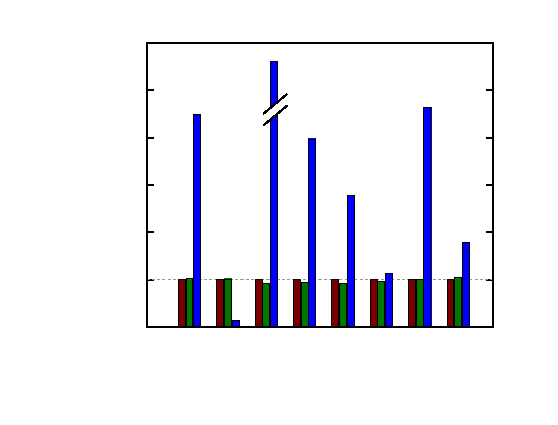
\includegraphics{numdist_insert}}%
    \gplfronttext
  \end{picture}%
\endgroup

\begin{tikzpicture}
    \node[draw,fill=darkred,minimum width=0.03in,minimum height=0.3in] at (0,0) {};
    \node at (0,0.77in) {\small\rotatebox{90}{Original cover tree}};
    \node[draw,fill=darkgreen,minimum width=0.03in,minimum height=0.3in] at (0.15in,0) {};
    \node at (0.15in,0.82in) {\small\rotatebox{90}{Simplified cover tree}};
    \node[draw,fill=blue,minimum width=0.03in,minimum height=0.3in] at (0.3in,0) {};
    \node at (0.3in,1.01in) {\small\rotatebox{90}{Nearest ancestor cover tree}};
    \node[minimum width=0.05in,minimum height=0.5in] at (0.45in,0) {};
    \node at (0.45in,0.6in) {\small\rotatebox{90}{}};
    \node at (0,-0.5in) {};
\end{tikzpicture}
\end{frame}

%%%%%%%%%%%%%%%%%%%%%%%%%%%%%%%%%%%%%%%%%%%%%%%%%%%%%%%%%%%%%%%%%%%%%%%%%%%%%%%%

\begin{frame}[fragile]{Comparing cover trees on \emph{construction and query} time}
\centering
\graphicspath{{slides/paperimg/}}
% GNUPLOT: LaTeX picture with Postscript
\begingroup
  \makeatletter
  \providecommand\color[2][]{%
    \GenericError{(gnuplot) \space\space\space\@spaces}{%
      Package color not loaded in conjunction with
      terminal option `colourtext'%
    }{See the gnuplot documentation for explanation.%
    }{Either use 'blacktext' in gnuplot or load the package
      color.sty in LaTeX.}%
    \renewcommand\color[2][]{}%
  }%
  \providecommand\includegraphics[2][]{%
    \GenericError{(gnuplot) \space\space\space\@spaces}{%
      Package graphicx or graphics not loaded%
    }{See the gnuplot documentation for explanation.%
    }{The gnuplot epslatex terminal needs graphicx.sty or graphics.sty.}%
    \renewcommand\includegraphics[2][]{}%
  }%
  \providecommand\rotatebox[2]{#2}%
  \@ifundefined{ifGPcolor}{%
    \newif\ifGPcolor
    \GPcolortrue
  }{}%
  \@ifundefined{ifGPblacktext}{%
    \newif\ifGPblacktext
    \GPblacktextfalse
  }{}%
  % define a \g@addto@macro without @ in the name:
  \let\gplgaddtomacro\g@addto@macro
  % define empty templates for all commands taking text:
  \gdef\gplbacktext{}%
  \gdef\gplfronttext{}%
  \makeatother
  \ifGPblacktext
    % no textcolor at all
    \def\colorrgb#1{}%
    \def\colorgray#1{}%
  \else
    % gray or color?
    \ifGPcolor
      \def\colorrgb#1{\color[rgb]{#1}}%
      \def\colorgray#1{\color[gray]{#1}}%
      \expandafter\def\csname LTw\endcsname{\color{white}}%
      \expandafter\def\csname LTb\endcsname{\color{black}}%
      \expandafter\def\csname LTa\endcsname{\color{black}}%
      \expandafter\def\csname LT0\endcsname{\color[rgb]{1,0,0}}%
      \expandafter\def\csname LT1\endcsname{\color[rgb]{0,1,0}}%
      \expandafter\def\csname LT2\endcsname{\color[rgb]{0,0,1}}%
      \expandafter\def\csname LT3\endcsname{\color[rgb]{1,0,1}}%
      \expandafter\def\csname LT4\endcsname{\color[rgb]{0,1,1}}%
      \expandafter\def\csname LT5\endcsname{\color[rgb]{1,1,0}}%
      \expandafter\def\csname LT6\endcsname{\color[rgb]{0,0,0}}%
      \expandafter\def\csname LT7\endcsname{\color[rgb]{1,0.3,0}}%
      \expandafter\def\csname LT8\endcsname{\color[rgb]{0.5,0.5,0.5}}%
    \else
      % gray
      \def\colorrgb#1{\color{black}}%
      \def\colorgray#1{\color[gray]{#1}}%
      \expandafter\def\csname LTw\endcsname{\color{white}}%
      \expandafter\def\csname LTb\endcsname{\color{black}}%
      \expandafter\def\csname LTa\endcsname{\color{black}}%
      \expandafter\def\csname LT0\endcsname{\color{black}}%
      \expandafter\def\csname LT1\endcsname{\color{black}}%
      \expandafter\def\csname LT2\endcsname{\color{black}}%
      \expandafter\def\csname LT3\endcsname{\color{black}}%
      \expandafter\def\csname LT4\endcsname{\color{black}}%
      \expandafter\def\csname LT5\endcsname{\color{black}}%
      \expandafter\def\csname LT6\endcsname{\color{black}}%
      \expandafter\def\csname LT7\endcsname{\color{black}}%
      \expandafter\def\csname LT8\endcsname{\color{black}}%
    \fi
  \fi
  \setlength{\unitlength}{0.0500bp}%
  \begin{picture}(5040.00,3772.00)%
    \gplgaddtomacro\gplbacktext{%
      \csname LTb\endcsname%
      \put(1122,780){\makebox(0,0)[r]{\strut{} 0}}%
      \put(1122,1235){\makebox(0,0)[r]{\strut{} 0.2}}%
      \put(1122,1689){\makebox(0,0)[r]{\strut{} 0.4}}%
      \put(1122,2144){\makebox(0,0)[r]{\strut{} 0.6}}%
      \put(1122,2598){\makebox(0,0)[r]{\strut{} 0.8}}%
      \put(1122,3052){\makebox(0,0)[r]{\strut{} 1}}%
      \put(1122,3507){\makebox(0,0)[r]{\strut{} 1.2}}%
      \put(1622,648){\rotatebox{-45}{\makebox(0,0)[l]{\strut{}yearpredict}}}%
      \put(1991,648){\rotatebox{-45}{\makebox(0,0)[l]{\strut{}twitter}}}%
      \put(2359,648){\rotatebox{-45}{\makebox(0,0)[l]{\strut{}tinyImages}}}%
      \put(2728,648){\rotatebox{-45}{\makebox(0,0)[l]{\strut{}mnist}}}%
      \put(3096,648){\rotatebox{-45}{\makebox(0,0)[l]{\strut{}corel}}}%
      \put(3465,648){\rotatebox{-45}{\makebox(0,0)[l]{\strut{}covtype}}}%
      \put(3833,648){\rotatebox{-45}{\makebox(0,0)[l]{\strut{}artificial40}}}%
      \put(4202,648){\rotatebox{-45}{\makebox(0,0)[l]{\strut{}faces}}}%
      \put(176,2143){\rotatebox{-270}{\makebox(0,0){\strut{}number of distance comparisons}}}%
      \put(396,2143){\rotatebox{-270}{\makebox(0,0){\strut{}in tree \emph{construction} and \emph{query}}}}%
      \put(616,2143){\rotatebox{-270}{\makebox(0,0){\strut{}(normalized by $n^2$)}}}%
    }%
    \gplgaddtomacro\gplfronttext{%
    }%
    \gplbacktext
    \put(0,0){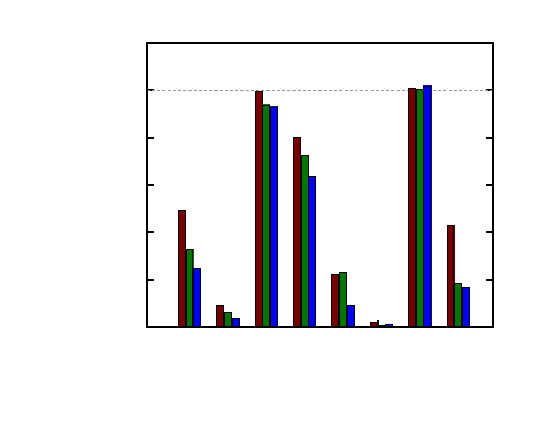
\includegraphics{numdist}}%
    \gplfronttext
  \end{picture}%
\endgroup

\begin{tikzpicture}
    \node[draw,fill=darkred,minimum width=0.03in,minimum height=0.3in] at (0,0) {};
    \node at (0,0.77in) {\small\rotatebox{90}{Original cover tree}};
    \node[draw,fill=darkgreen,minimum width=0.03in,minimum height=0.3in] at (0.15in,0) {};
    \node at (0.15in,0.82in) {\small\rotatebox{90}{Simplified cover tree}};
    \node[draw,fill=blue,minimum width=0.03in,minimum height=0.3in] at (0.3in,0) {};
    \node at (0.3in,1.01in) {\small\rotatebox{90}{Nearest ancestor cover tree}};
    \node[minimum width=0.05in,minimum height=0.5in] at (0.45in,0) {};
    \node at (0.45in,0.6in) {\small\rotatebox{90}{}};
    \node at (0,-0.5in) {};
\end{tikzpicture}
\end{frame}

%%%%%%%%%%%%%%%%%%%%%%%%%%%%%%%%%%%%%%%%%%%%%%%%%%%%%%%%%%%%%%%%%%%%%%%%%%%%%%%%

\begin{frame}[fragile]{All of the cover trees scale similarly}

This experiment uses the protein data and the random walk graph kernel.
\vspace{0.15in}

{
\centering
\graphicspath{{slides/paperimg/}}
% GNUPLOT: LaTeX picture with Postscript
\begingroup
  \makeatletter
  \providecommand\color[2][]{%
    \GenericError{(gnuplot) \space\space\space\@spaces}{%
      Package color not loaded in conjunction with
      terminal option `colourtext'%
    }{See the gnuplot documentation for explanation.%
    }{Either use 'blacktext' in gnuplot or load the package
      color.sty in LaTeX.}%
    \renewcommand\color[2][]{}%
  }%
  \providecommand\includegraphics[2][]{%
    \GenericError{(gnuplot) \space\space\space\@spaces}{%
      Package graphicx or graphics not loaded%
    }{See the gnuplot documentation for explanation.%
    }{The gnuplot epslatex terminal needs graphicx.sty or graphics.sty.}%
    \renewcommand\includegraphics[2][]{}%
  }%
  \providecommand\rotatebox[2]{#2}%
  \@ifundefined{ifGPcolor}{%
    \newif\ifGPcolor
    \GPcolortrue
  }{}%
  \@ifundefined{ifGPblacktext}{%
    \newif\ifGPblacktext
    \GPblacktextfalse
  }{}%
  % define a \g@addto@macro without @ in the name:
  \let\gplgaddtomacro\g@addto@macro
  % define empty templates for all commands taking text:
  \gdef\gplbacktext{}%
  \gdef\gplfronttext{}%
  \makeatother
  \ifGPblacktext
    % no textcolor at all
    \def\colorrgb#1{}%
    \def\colorgray#1{}%
  \else
    % gray or color?
    \ifGPcolor
      \def\colorrgb#1{\color[rgb]{#1}}%
      \def\colorgray#1{\color[gray]{#1}}%
      \expandafter\def\csname LTw\endcsname{\color{white}}%
      \expandafter\def\csname LTb\endcsname{\color{black}}%
      \expandafter\def\csname LTa\endcsname{\color{black}}%
      \expandafter\def\csname LT0\endcsname{\color[rgb]{1,0,0}}%
      \expandafter\def\csname LT1\endcsname{\color[rgb]{0,1,0}}%
      \expandafter\def\csname LT2\endcsname{\color[rgb]{0,0,1}}%
      \expandafter\def\csname LT3\endcsname{\color[rgb]{1,0,1}}%
      \expandafter\def\csname LT4\endcsname{\color[rgb]{0,1,1}}%
      \expandafter\def\csname LT5\endcsname{\color[rgb]{1,1,0}}%
      \expandafter\def\csname LT6\endcsname{\color[rgb]{0,0,0}}%
      \expandafter\def\csname LT7\endcsname{\color[rgb]{1,0.3,0}}%
      \expandafter\def\csname LT8\endcsname{\color[rgb]{0.5,0.5,0.5}}%
    \else
      % gray
      \def\colorrgb#1{\color{black}}%
      \def\colorgray#1{\color[gray]{#1}}%
      \expandafter\def\csname LTw\endcsname{\color{white}}%
      \expandafter\def\csname LTb\endcsname{\color{black}}%
      \expandafter\def\csname LTa\endcsname{\color{black}}%
      \expandafter\def\csname LT0\endcsname{\color{black}}%
      \expandafter\def\csname LT1\endcsname{\color{black}}%
      \expandafter\def\csname LT2\endcsname{\color{black}}%
      \expandafter\def\csname LT3\endcsname{\color{black}}%
      \expandafter\def\csname LT4\endcsname{\color{black}}%
      \expandafter\def\csname LT5\endcsname{\color{black}}%
      \expandafter\def\csname LT6\endcsname{\color{black}}%
      \expandafter\def\csname LT7\endcsname{\color{black}}%
      \expandafter\def\csname LT8\endcsname{\color{black}}%
    \fi
  \fi
  \setlength{\unitlength}{0.0500bp}%
  \begin{picture}(5040.00,3772.00)%
    \gplgaddtomacro\gplbacktext{%
      \csname LTb\endcsname%
      \put(1298,704){\makebox(0,0)[r]{\strut{} 0}}%
      \put(1298,1054){\makebox(0,0)[r]{\strut{} 200}}%
      \put(1298,1405){\makebox(0,0)[r]{\strut{} 400}}%
      \put(1298,1755){\makebox(0,0)[r]{\strut{} 600}}%
      \put(1298,2106){\makebox(0,0)[r]{\strut{} 800}}%
      \put(1298,2456){\makebox(0,0)[r]{\strut{} 1000}}%
      \put(1298,2806){\makebox(0,0)[r]{\strut{} 1200}}%
      \put(1298,3157){\makebox(0,0)[r]{\strut{} 1400}}%
      \put(1298,3507){\makebox(0,0)[r]{\strut{} 1600}}%
      \put(1430,484){\makebox(0,0){\strut{} 0}}%
      \put(2073,484){\makebox(0,0){\strut{} 50}}%
      \put(2715,484){\makebox(0,0){\strut{} 100}}%
      \put(3358,484){\makebox(0,0){\strut{} 150}}%
      \put(4000,484){\makebox(0,0){\strut{} 200}}%
      \put(4643,484){\makebox(0,0){\strut{} 250}}%
      \put(176,2105){\rotatebox{-270}{\makebox(0,0){\strut{}total distance comparisons (millions)}}}%
      \put(396,2105){\rotatebox{-270}{\makebox(0,0){\strut{}on \emph{construction} and \emph{query}}}}%
      \put(3036,154){\makebox(0,0){\strut{}number of data points (thousands)}}%
    }%
    \gplgaddtomacro\gplfronttext{%
    }%
    \gplbacktext
    \put(0,0){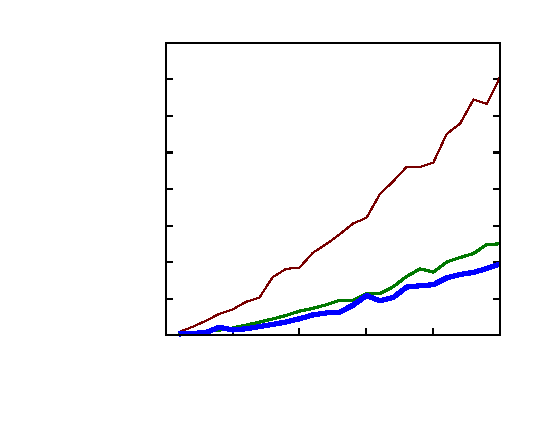
\includegraphics{protein-simple}}%
    \gplfronttext
  \end{picture}%
\endgroup

\begin{tikzpicture}
    \node[draw,fill=darkred,minimum width=0.03in,minimum height=0.3in] at (0,0) {};
    \node at (0,0.77in) {\small\rotatebox{90}{Original cover tree}};
    \node[draw,fill=darkgreen,minimum width=0.03in,minimum height=0.3in] at (0.15in,0) {};
    \node at (0.15in,0.82in) {\small\rotatebox{90}{Simplified cover tree}};
    \node[draw,fill=blue,minimum width=0.03in,minimum height=0.3in] at (0.3in,0) {};
    \node at (0.3in,1.01in) {\small\rotatebox{90}{Nearest ancestor cover tree}};
    \node[minimum width=0.05in,minimum height=0.5in] at (0.45in,0) {};
    %\node at (0.6in,0.7in) {\small\rotatebox{90}{ dotted lines: construction only}};
    %\node at (0.75in,0.81in) {\small\rotatebox{90}{ solid lines: construction and query}};
    \node at (0,-0.5in) {};
\end{tikzpicture}
}

\end{frame}

\begin{frame}[fragile]{Cache oblivious cover tree}

%RAM model is a lie
%
%\vspace{0.1in}
Need to consider cache accesses for fast, modern data structures

%\vspace{0.1in}
%In a \emph{cache oblivious} data structure, the programmer doesn't need to know any details about the underlying hardware
%
\begin{center}
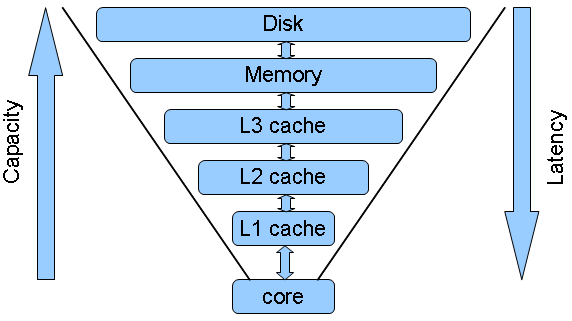
\includegraphics[width=10cm]{slides/cpu_cache_structure}
\end{center}

{\tiny image from: \url{http://1024cores.net} }
\end{frame}

%%%%%%%%%%%%%%%%%%%%%%%%%%%%%%%%%%%%%%%%%%%%%%%%%%%%%%%%%%%%%%%%%%%%%%%%%%%%%%%%

\begin{frame}[fragile]{Cache oblivious cover tree}

%The trick: use the van Emde Boas tree layout
Arrange nodes in memory according to a preorder traversal of the tree

(van Emde Boas \emph{et al.}, 1966; Demaine, 2002)
\vspace{0.1in}

\begin{center}
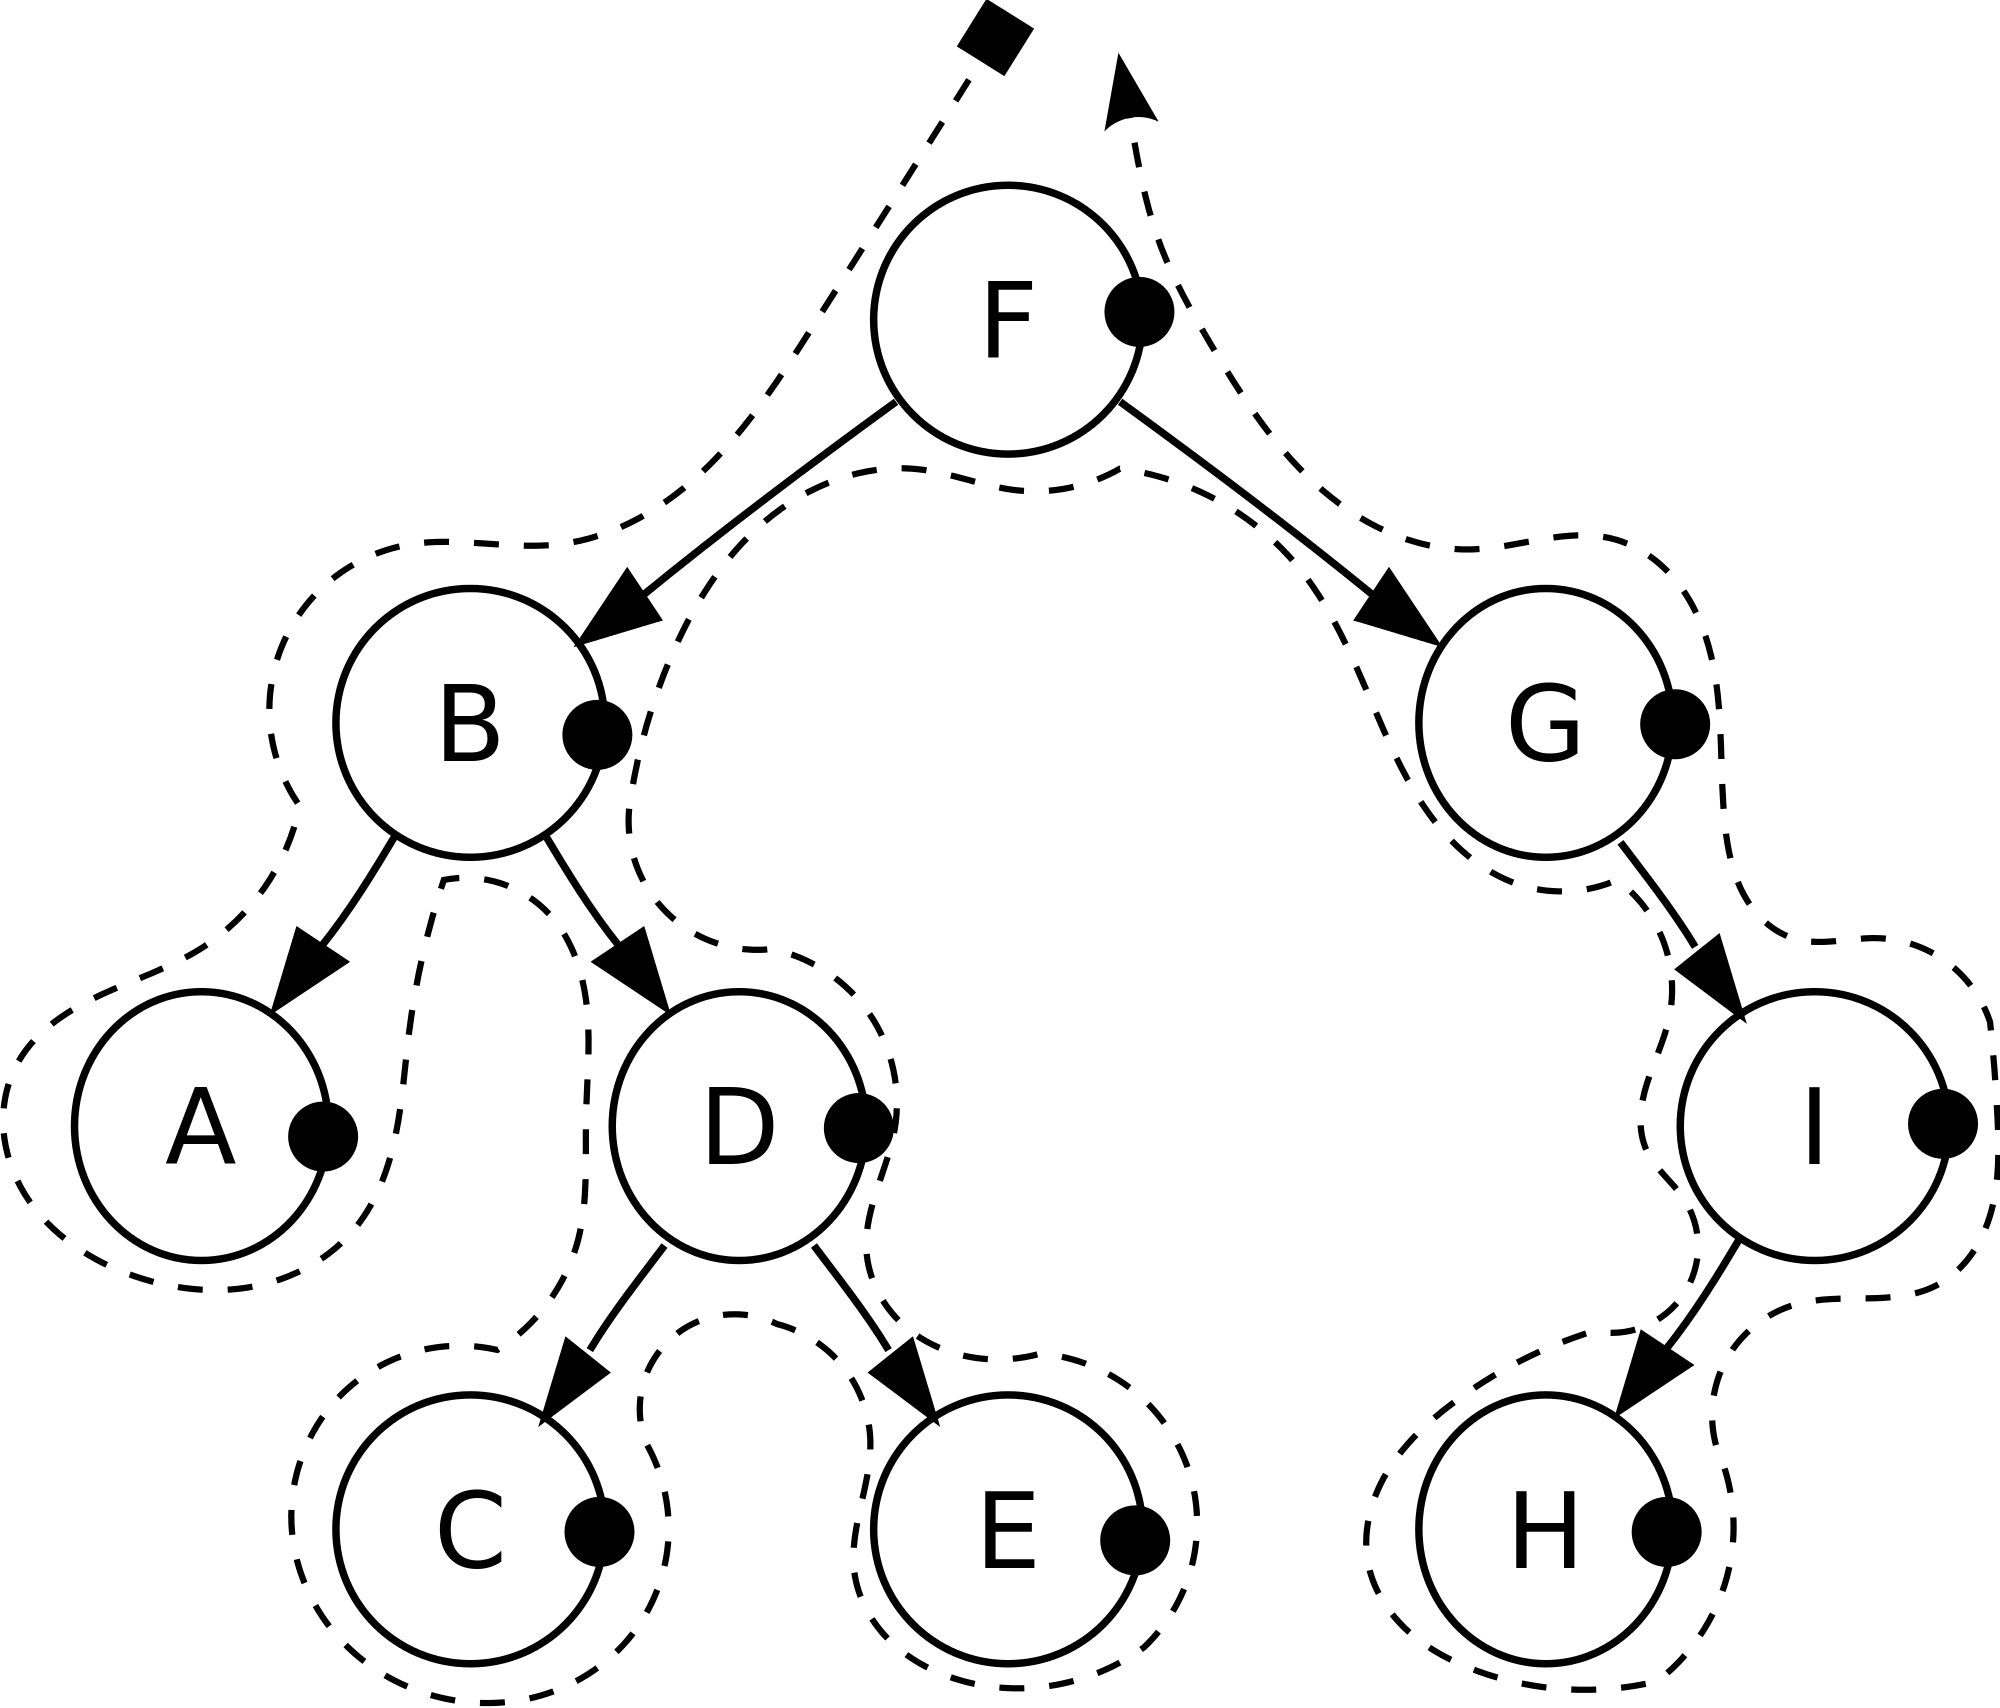
\includegraphics[width=6cm]{slides/preorder.png}
\end{center}

{\tiny image from: Wikipedia}
%(nodes arranged in memory according to a pre-order depth first traversal)
%
%\vspace{-0.1in}
%%{
%%\centering
%\begin{center}
%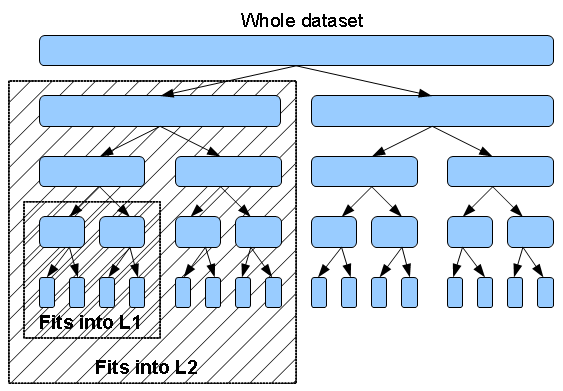
\includegraphics[width=8cm]{slides/cache_oblivious_divide}
%\end{center}
%%}
%
%\vspace{-0.1in}
%Optimal cache performance without any knowledge of the architecture
%\vspace{0.15in}

%source: 1024cores.net

\end{frame}

%%%%%%%%%%%%%%%%%%%%%%%%%%%%%%%%%%%%%%%%%%%%%%%%%%%%%%%%%%%%%%%%%%%%%%%%%%%%%%%%

\begin{frame}[fragile]{The cache efficiency of three cover tree implementations}

\centering
\graphicspath{{slides/paperimg/}}
% GNUPLOT: LaTeX picture with Postscript
\begingroup
  \makeatletter
  \providecommand\color[2][]{%
    \GenericError{(gnuplot) \space\space\space\@spaces}{%
      Package color not loaded in conjunction with
      terminal option `colourtext'%
    }{See the gnuplot documentation for explanation.%
    }{Either use 'blacktext' in gnuplot or load the package
      color.sty in LaTeX.}%
    \renewcommand\color[2][]{}%
  }%
  \providecommand\includegraphics[2][]{%
    \GenericError{(gnuplot) \space\space\space\@spaces}{%
      Package graphicx or graphics not loaded%
    }{See the gnuplot documentation for explanation.%
    }{The gnuplot epslatex terminal needs graphicx.sty or graphics.sty.}%
    \renewcommand\includegraphics[2][]{}%
  }%
  \providecommand\rotatebox[2]{#2}%
  \@ifundefined{ifGPcolor}{%
    \newif\ifGPcolor
    \GPcolortrue
  }{}%
  \@ifundefined{ifGPblacktext}{%
    \newif\ifGPblacktext
    \GPblacktextfalse
  }{}%
  % define a \g@addto@macro without @ in the name:
  \let\gplgaddtomacro\g@addto@macro
  % define empty templates for all commands taking text:
  \gdef\gplbacktext{}%
  \gdef\gplfronttext{}%
  \makeatother
  \ifGPblacktext
    % no textcolor at all
    \def\colorrgb#1{}%
    \def\colorgray#1{}%
  \else
    % gray or color?
    \ifGPcolor
      \def\colorrgb#1{\color[rgb]{#1}}%
      \def\colorgray#1{\color[gray]{#1}}%
      \expandafter\def\csname LTw\endcsname{\color{white}}%
      \expandafter\def\csname LTb\endcsname{\color{black}}%
      \expandafter\def\csname LTa\endcsname{\color{black}}%
      \expandafter\def\csname LT0\endcsname{\color[rgb]{1,0,0}}%
      \expandafter\def\csname LT1\endcsname{\color[rgb]{0,1,0}}%
      \expandafter\def\csname LT2\endcsname{\color[rgb]{0,0,1}}%
      \expandafter\def\csname LT3\endcsname{\color[rgb]{1,0,1}}%
      \expandafter\def\csname LT4\endcsname{\color[rgb]{0,1,1}}%
      \expandafter\def\csname LT5\endcsname{\color[rgb]{1,1,0}}%
      \expandafter\def\csname LT6\endcsname{\color[rgb]{0,0,0}}%
      \expandafter\def\csname LT7\endcsname{\color[rgb]{1,0.3,0}}%
      \expandafter\def\csname LT8\endcsname{\color[rgb]{0.5,0.5,0.5}}%
    \else
      % gray
      \def\colorrgb#1{\color{black}}%
      \def\colorgray#1{\color[gray]{#1}}%
      \expandafter\def\csname LTw\endcsname{\color{white}}%
      \expandafter\def\csname LTb\endcsname{\color{black}}%
      \expandafter\def\csname LTa\endcsname{\color{black}}%
      \expandafter\def\csname LT0\endcsname{\color{black}}%
      \expandafter\def\csname LT1\endcsname{\color{black}}%
      \expandafter\def\csname LT2\endcsname{\color{black}}%
      \expandafter\def\csname LT3\endcsname{\color{black}}%
      \expandafter\def\csname LT4\endcsname{\color{black}}%
      \expandafter\def\csname LT5\endcsname{\color{black}}%
      \expandafter\def\csname LT6\endcsname{\color{black}}%
      \expandafter\def\csname LT7\endcsname{\color{black}}%
      \expandafter\def\csname LT8\endcsname{\color{black}}%
    \fi
  \fi
  \setlength{\unitlength}{0.0500bp}%
  \begin{picture}(5040.00,3772.00)%
    \gplgaddtomacro\gplbacktext{%
      \csname LTb\endcsname%
      \put(1166,780){\makebox(0,0)[r]{\strut{} 0}}%
      \put(1166,1325){\makebox(0,0)[r]{\strut{} 0.2}}%
      \put(1166,1871){\makebox(0,0)[r]{\strut{} 0.4}}%
      \put(1166,2416){\makebox(0,0)[r]{\strut{} 0.6}}%
      \put(1166,2962){\makebox(0,0)[r]{\strut{} 0.8}}%
      \put(1166,3507){\makebox(0,0)[r]{\strut{} 1}}%
      \put(1661,648){\rotatebox{-45}{\makebox(0,0)[l]{\strut{}yearpredict}}}%
      \put(2023,648){\rotatebox{-45}{\makebox(0,0)[l]{\strut{}twitter}}}%
      \put(2386,648){\rotatebox{-45}{\makebox(0,0)[l]{\strut{}tinyImages}}}%
      \put(2748,648){\rotatebox{-45}{\makebox(0,0)[l]{\strut{}mnist}}}%
      \put(3111,648){\rotatebox{-45}{\makebox(0,0)[l]{\strut{}corel}}}%
      \put(3473,648){\rotatebox{-45}{\makebox(0,0)[l]{\strut{}covtype}}}%
      \put(3836,648){\rotatebox{-45}{\makebox(0,0)[l]{\strut{}artificial40}}}%
      \put(4198,648){\rotatebox{-45}{\makebox(0,0)[l]{\strut{}faces}}}%
      \put(176,2143){\rotatebox{-270}{\makebox(0,0){\strut{}cache miss rate}}}%
      \put(396,2143){\rotatebox{-270}{\makebox(0,0){\strut{}(cache misses / cache accesses)}}}%
    }%
    \gplgaddtomacro\gplfronttext{%
    }%
    \gplbacktext
    \put(0,0){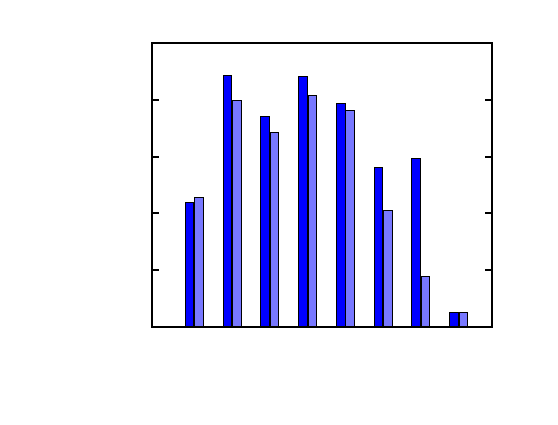
\includegraphics{cache-hlearn}}%
    \gplfronttext
  \end{picture}%
\endgroup

\definecolor{colorOrig}{RGB}{102,51,0}
\definecolor{colorMlpack}{RGB}{204,153,0}
\begin{tikzpicture}
    %\node[draw,fill=colorOrig,minimum width=0.05in,minimum height=0.3in] at (0,0) {};
    %\node at (0,0.79in) {\small\rotatebox{90}{Reference cover tree}};
    %\node[draw,fill=colorMlpack,minimum width=0.05in,minimum height=0.3in] at (0.15in,0) {};
    %\node at (0.15in,0.79in) {\small\rotatebox{90}{MLPack's cover tree}};
    %\node[draw,fill=blue,minimum width=0.05in,minimum height=0.3in] at (0.3in,0) {};
    %\node at (0.3in,0.98in) {\small\rotatebox{90}{Our cover tree (unpacked)}};
    %\node[draw,fill=lightblue,minimum width=0.05in,minimum height=0.3in] at (0.45in,0) {};
    %\node at (0.45in,0.91in) {\small\rotatebox{90}{Our cover tree (packed)}};
    \node[draw,fill=blue,minimum width=0.05in,minimum height=0.3in] at (0.3in,0) {};
    \node at (0.3in,0.98in) {\small\rotatebox{90}{Without van embde boas }};
    \node[draw,fill=lightblue,minimum width=0.05in,minimum height=0.3in] at (0.45in,0) {};
    \node at (0.45in,0.88in) {\small\rotatebox{90}{With van embde boas }};
    \node at (0,-0.475in) {};
\end{tikzpicture}

\vspace{0.15in}
Measured using Linux's \lstinline{perf stat} utility on an Amazon AWS instance
\end{frame}

%%%%%%%%%%%%%%%%%%%%%%%%%%%%%%%%%%%%%%%%%%%%%%%%%%%%%%%%%%%%%%%%%%%%%%%%%%%%%%%%
%
%\begin{frame}[fragile]{The cache efficiency of three cover tree implementations}
%
%\centering
%\graphicspath{{slides/paperimg/}}
%% GNUPLOT: LaTeX picture with Postscript
\begingroup
  \makeatletter
  \providecommand\color[2][]{%
    \GenericError{(gnuplot) \space\space\space\@spaces}{%
      Package color not loaded in conjunction with
      terminal option `colourtext'%
    }{See the gnuplot documentation for explanation.%
    }{Either use 'blacktext' in gnuplot or load the package
      color.sty in LaTeX.}%
    \renewcommand\color[2][]{}%
  }%
  \providecommand\includegraphics[2][]{%
    \GenericError{(gnuplot) \space\space\space\@spaces}{%
      Package graphicx or graphics not loaded%
    }{See the gnuplot documentation for explanation.%
    }{The gnuplot epslatex terminal needs graphicx.sty or graphics.sty.}%
    \renewcommand\includegraphics[2][]{}%
  }%
  \providecommand\rotatebox[2]{#2}%
  \@ifundefined{ifGPcolor}{%
    \newif\ifGPcolor
    \GPcolortrue
  }{}%
  \@ifundefined{ifGPblacktext}{%
    \newif\ifGPblacktext
    \GPblacktextfalse
  }{}%
  % define a \g@addto@macro without @ in the name:
  \let\gplgaddtomacro\g@addto@macro
  % define empty templates for all commands taking text:
  \gdef\gplbacktext{}%
  \gdef\gplfronttext{}%
  \makeatother
  \ifGPblacktext
    % no textcolor at all
    \def\colorrgb#1{}%
    \def\colorgray#1{}%
  \else
    % gray or color?
    \ifGPcolor
      \def\colorrgb#1{\color[rgb]{#1}}%
      \def\colorgray#1{\color[gray]{#1}}%
      \expandafter\def\csname LTw\endcsname{\color{white}}%
      \expandafter\def\csname LTb\endcsname{\color{black}}%
      \expandafter\def\csname LTa\endcsname{\color{black}}%
      \expandafter\def\csname LT0\endcsname{\color[rgb]{1,0,0}}%
      \expandafter\def\csname LT1\endcsname{\color[rgb]{0,1,0}}%
      \expandafter\def\csname LT2\endcsname{\color[rgb]{0,0,1}}%
      \expandafter\def\csname LT3\endcsname{\color[rgb]{1,0,1}}%
      \expandafter\def\csname LT4\endcsname{\color[rgb]{0,1,1}}%
      \expandafter\def\csname LT5\endcsname{\color[rgb]{1,1,0}}%
      \expandafter\def\csname LT6\endcsname{\color[rgb]{0,0,0}}%
      \expandafter\def\csname LT7\endcsname{\color[rgb]{1,0.3,0}}%
      \expandafter\def\csname LT8\endcsname{\color[rgb]{0.5,0.5,0.5}}%
    \else
      % gray
      \def\colorrgb#1{\color{black}}%
      \def\colorgray#1{\color[gray]{#1}}%
      \expandafter\def\csname LTw\endcsname{\color{white}}%
      \expandafter\def\csname LTb\endcsname{\color{black}}%
      \expandafter\def\csname LTa\endcsname{\color{black}}%
      \expandafter\def\csname LT0\endcsname{\color{black}}%
      \expandafter\def\csname LT1\endcsname{\color{black}}%
      \expandafter\def\csname LT2\endcsname{\color{black}}%
      \expandafter\def\csname LT3\endcsname{\color{black}}%
      \expandafter\def\csname LT4\endcsname{\color{black}}%
      \expandafter\def\csname LT5\endcsname{\color{black}}%
      \expandafter\def\csname LT6\endcsname{\color{black}}%
      \expandafter\def\csname LT7\endcsname{\color{black}}%
      \expandafter\def\csname LT8\endcsname{\color{black}}%
    \fi
  \fi
  \setlength{\unitlength}{0.0500bp}%
  \begin{picture}(5040.00,3772.00)%
    \gplgaddtomacro\gplbacktext{%
      \csname LTb\endcsname%
      \put(1166,780){\makebox(0,0)[r]{\strut{} 0}}%
      \put(1166,1325){\makebox(0,0)[r]{\strut{} 0.2}}%
      \put(1166,1871){\makebox(0,0)[r]{\strut{} 0.4}}%
      \put(1166,2416){\makebox(0,0)[r]{\strut{} 0.6}}%
      \put(1166,2962){\makebox(0,0)[r]{\strut{} 0.8}}%
      \put(1166,3507){\makebox(0,0)[r]{\strut{} 1}}%
      \put(1661,648){\rotatebox{-45}{\makebox(0,0)[l]{\strut{}yearpredict}}}%
      \put(2023,648){\rotatebox{-45}{\makebox(0,0)[l]{\strut{}twitter}}}%
      \put(2386,648){\rotatebox{-45}{\makebox(0,0)[l]{\strut{}tinyImages}}}%
      \put(2748,648){\rotatebox{-45}{\makebox(0,0)[l]{\strut{}mnist}}}%
      \put(3111,648){\rotatebox{-45}{\makebox(0,0)[l]{\strut{}corel}}}%
      \put(3473,648){\rotatebox{-45}{\makebox(0,0)[l]{\strut{}covtype}}}%
      \put(3836,648){\rotatebox{-45}{\makebox(0,0)[l]{\strut{}artificial40}}}%
      \put(4198,648){\rotatebox{-45}{\makebox(0,0)[l]{\strut{}faces}}}%
      \put(176,2143){\rotatebox{-270}{\makebox(0,0){\strut{}stalled CPU cycle rate}}}%
      \put(396,2143){\rotatebox{-270}{\makebox(0,0){\strut{}(stalled cycles / total cycles)}}}%
    }%
    \gplgaddtomacro\gplfronttext{%
    }%
    \gplbacktext
    \put(0,0){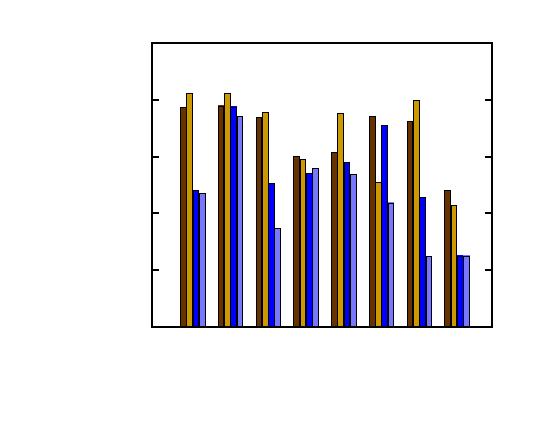
\includegraphics{stalled-front}}%
    \gplfronttext
  \end{picture}%
\endgroup

%\definecolor{colorOrig}{RGB}{102,51,0}
%\definecolor{colorMlpack}{RGB}{204,153,0}
%\begin{tikzpicture}
    %\node[draw,fill=colorOrig,minimum width=0.05in,minimum height=0.3in] at (0,0) {};
    %\node at (0,0.79in) {\small\rotatebox{90}{Reference cover tree}};
    %\node[draw,fill=colorMlpack,minimum width=0.05in,minimum height=0.3in] at (0.15in,0) {};
    %\node at (0.15in,0.79in) {\small\rotatebox{90}{MLPack's cover tree}};
    %\node[draw,fill=blue,minimum width=0.05in,minimum height=0.3in] at (0.3in,0) {};
    %\node at (0.3in,0.98in) {\small\rotatebox{90}{Our cover tree (unpacked)}};
    %\node[draw,fill=lightblue,minimum width=0.05in,minimum height=0.3in] at (0.45in,0) {};
    %\node at (0.45in,0.91in) {\small\rotatebox{90}{Our cover tree (packed)}};
    %\node at (0,-0.475in) {};
%\end{tikzpicture}
%
%\vspace{0.15in}
%Measured using Linux's \lstinline{perf stat} utility on an Amazon AWS instance
%\end{frame}

\begin{frame}[fragile]{Merging cover trees}

Merging cover trees gives us a parallel tree construction algorithm

\vspace{0.15in}

Sometimes, merging cover trees is \textbf{easy}:

\begin{center}
\begin{tikzpicture}
    [ draw
    , every node/.style={minimum size=10mm,fill=white}
    , level/.style={sibling distance = 23mm/#1, level distance=12mm}
    %,    level distance = 1.5cm}
    , sibling distance=8mm
    ]
\draw (-2.3,0) -- (8.6,0)[dotted];
\draw (-2.3,-12mm) -- (8.6,-12mm)[dotted];
\draw (-2.3,-24mm) -- (8.6,-24mm)[dotted];
\node[shape=circle,draw] at (0,0) {10}
    child { node[circle,draw] {8}
        child { node[circle,draw] {7}  }
        child { node[circle,draw] {9} }
        }
    child [color=white] {}
    %child { node[circle,draw] {12}
        %child { node[circle,draw] {9}  }
        %child { node[circle,draw] {13} }
        %}
    ;
\node[shape=circle,draw,fill=lightgreen] at (5,-12mm) {12}
    %child { node[circle,draw] {8}
        %child { node[circle,draw] {7}  }
        %child { node[circle,draw,fill=lightgreen,line width=1pt] {9} }
        %}
    %child { node[circle,draw] {12}
        child { node[circle,draw] {11}  }
        child { node[circle,draw] {13} }
        %}
    ;
\node[fill=none] at (8,3mm) {level 3};
\node[fill=none] at (8,-9mm) {level 2};
\node[fill=none] at (8,-21mm) {level 1};
\end{tikzpicture}
\end{center}

\vspace{0.1in}
No runtime bound on the merge operation, but it is fast in practice

%\vspace{0.1in}
%But, if the runtime is $o(n)$, then we get an algorithm for tree construction that takes time $O(n)$
\end{frame}

%%%%%%%%%%%%%%%%%%%%%%%%%%%%%%%%%%%%%%%%%%%%%%%%%%%%%%%%%%%%%%%%%%%%%%%%%%%%%%%%

\begin{frame}[fragile]{Merging cover trees}

Merging cover trees gives us a parallel tree construction algorithm

\vspace{0.15in}

Sometimes, merging cover trees is \textbf{hard}:

\begin{center}
\begin{tikzpicture}
    [ draw
    , every node/.style={minimum size=10mm,fill=white}
    , level/.style={sibling distance = 23mm/#1, level distance=12mm}
    %,    level distance = 1.5cm}
    , sibling distance=8mm
    ]
\draw (-2.3,0) -- (8.6,0)[dotted];
\draw (-2.3,-12mm) -- (8.6,-12mm)[dotted];
\draw (-2.3,-24mm) -- (8.6,-24mm)[dotted];
\node[shape=circle,draw] at (0,0) {10}
    child { node[circle,draw] {8}
        child { node[circle,draw] {7}  }
        child { node[circle,draw] {9} }
        }
    child [color=white] {}
    %child { node[circle,draw] {12}
        %child { node[circle,draw] {9}  }
        %child { node[circle,draw] {13} }
        %}
    ;
\node[shape=circle,draw,fill=lightred] at (5,-12mm) {11.5}
    %child { node[circle,draw] {8}
        %child { node[circle,draw] {7}  }
        %child { node[circle,draw,fill=lightgreen,line width=1pt] {9} }
        %}
    %child { node[circle,draw] {12}
        child { node[circle,draw] {11}  }
        child { node[circle,draw] {13} }
        %}
    ;
\node[fill=none] at (8,3mm) {level 3};
\node[fill=none] at (8,-9mm) {level 2};
\node[fill=none] at (8,-21mm) {level 1};
\end{tikzpicture}
\end{center}

\vspace{0.1in}
No runtime bound on the merge operation, but it is fast in practice

%\vspace{0.1in}
%But, if the runtime is $o(n)$, then we get an algorithm for tree construction that takes time $O(n)$
\end{frame}

%%%%%%%%%%%%%%%%%%%%%%%%%%%%%%%%%%%%%%%%%%%%%%%%%%%%%%%%%%%%%%%%%%%%%%%%%%%%%%%%

\begin{frame}[fragile]{The effect of parallel tree \emph{construction} on small datasets}
\begin{center}
\graphicspath{{slides/paperimg/}}
% GNUPLOT: LaTeX picture with Postscript
\begingroup
  \makeatletter
  \providecommand\color[2][]{%
    \GenericError{(gnuplot) \space\space\space\@spaces}{%
      Package color not loaded in conjunction with
      terminal option `colourtext'%
    }{See the gnuplot documentation for explanation.%
    }{Either use 'blacktext' in gnuplot or load the package
      color.sty in LaTeX.}%
    \renewcommand\color[2][]{}%
  }%
  \providecommand\includegraphics[2][]{%
    \GenericError{(gnuplot) \space\space\space\@spaces}{%
      Package graphicx or graphics not loaded%
    }{See the gnuplot documentation for explanation.%
    }{The gnuplot epslatex terminal needs graphicx.sty or graphics.sty.}%
    \renewcommand\includegraphics[2][]{}%
  }%
  \providecommand\rotatebox[2]{#2}%
  \@ifundefined{ifGPcolor}{%
    \newif\ifGPcolor
    \GPcolortrue
  }{}%
  \@ifundefined{ifGPblacktext}{%
    \newif\ifGPblacktext
    \GPblacktextfalse
  }{}%
  % define a \g@addto@macro without @ in the name:
  \let\gplgaddtomacro\g@addto@macro
  % define empty templates for all commands taking text:
  \gdef\gplbacktext{}%
  \gdef\gplfronttext{}%
  \makeatother
  \ifGPblacktext
    % no textcolor at all
    \def\colorrgb#1{}%
    \def\colorgray#1{}%
  \else
    % gray or color?
    \ifGPcolor
      \def\colorrgb#1{\color[rgb]{#1}}%
      \def\colorgray#1{\color[gray]{#1}}%
      \expandafter\def\csname LTw\endcsname{\color{white}}%
      \expandafter\def\csname LTb\endcsname{\color{black}}%
      \expandafter\def\csname LTa\endcsname{\color{black}}%
      \expandafter\def\csname LT0\endcsname{\color[rgb]{1,0,0}}%
      \expandafter\def\csname LT1\endcsname{\color[rgb]{0,1,0}}%
      \expandafter\def\csname LT2\endcsname{\color[rgb]{0,0,1}}%
      \expandafter\def\csname LT3\endcsname{\color[rgb]{1,0,1}}%
      \expandafter\def\csname LT4\endcsname{\color[rgb]{0,1,1}}%
      \expandafter\def\csname LT5\endcsname{\color[rgb]{1,1,0}}%
      \expandafter\def\csname LT6\endcsname{\color[rgb]{0,0,0}}%
      \expandafter\def\csname LT7\endcsname{\color[rgb]{1,0.3,0}}%
      \expandafter\def\csname LT8\endcsname{\color[rgb]{0.5,0.5,0.5}}%
    \else
      % gray
      \def\colorrgb#1{\color{black}}%
      \def\colorgray#1{\color[gray]{#1}}%
      \expandafter\def\csname LTw\endcsname{\color{white}}%
      \expandafter\def\csname LTb\endcsname{\color{black}}%
      \expandafter\def\csname LTa\endcsname{\color{black}}%
      \expandafter\def\csname LT0\endcsname{\color{black}}%
      \expandafter\def\csname LT1\endcsname{\color{black}}%
      \expandafter\def\csname LT2\endcsname{\color{black}}%
      \expandafter\def\csname LT3\endcsname{\color{black}}%
      \expandafter\def\csname LT4\endcsname{\color{black}}%
      \expandafter\def\csname LT5\endcsname{\color{black}}%
      \expandafter\def\csname LT6\endcsname{\color{black}}%
      \expandafter\def\csname LT7\endcsname{\color{black}}%
      \expandafter\def\csname LT8\endcsname{\color{black}}%
    \fi
  \fi
  \setlength{\unitlength}{0.0500bp}%
  \begin{picture}(5040.00,3772.00)%
    \gplgaddtomacro\gplbacktext{%
      \csname LTb\endcsname%
      \put(814,1129){\makebox(0,0)[r]{\strut{}$2^{-4}$}}%
      \csname LTb\endcsname%
      \put(814,1526){\makebox(0,0)[r]{\strut{}$2^{-3}$}}%
      \csname LTb\endcsname%
      \put(814,1922){\makebox(0,0)[r]{\strut{}$2^{-2}$}}%
      \csname LTb\endcsname%
      \put(814,2318){\makebox(0,0)[r]{\strut{}$2^{-1}$}}%
      \csname LTb\endcsname%
      \put(814,2714){\makebox(0,0)[r]{\strut{}$2^{+0}$}}%
      \csname LTb\endcsname%
      \put(814,3111){\makebox(0,0)[r]{\strut{}$2^{+1}$}}%
      \put(1539,601){\rotatebox{-45}{\makebox(0,0)[l]{\strut{}yearpredict}}}%
      \put(1539,381){\rotatebox{-45}{\makebox(0,0)[l]{\strut{}(77sec)}}}%
      \put(2242,601){\rotatebox{-45}{\makebox(0,0)[l]{\strut{}twitter}}}%
      \put(2242,381){\rotatebox{-45}{\makebox(0,0)[l]{\strut{}(107sec)}}}%
      \put(2945,601){\rotatebox{-45}{\makebox(0,0)[l]{\strut{}tinyImages}}}%
      \put(2945,381){\rotatebox{-45}{\makebox(0,0)[l]{\strut{}(65sec)}}}%
      \put(3648,601){\rotatebox{-45}{\makebox(0,0)[l]{\strut{}mnist}}}%
      \put(3648,381){\rotatebox{-45}{\makebox(0,0)[l]{\strut{}(12sec)}}}%
      \put(176,2120){\rotatebox{-270}{\makebox(0,0){\strut{}normalized tree \emph{construction} time}}}%
      \put(1464,2814){\makebox(0,0)[l]{\strut{}\tiny 1}}%
      \put(1570,2619){\makebox(0,0)[l]{\strut{}\tiny 2}}%
      \put(1667,2175){\makebox(0,0)[l]{\strut{}\tiny 4}}%
      \put(1763,1967){\makebox(0,0)[l]{\strut{}\tiny 8}}%
      \put(1860,1856){\makebox(0,0)[l]{\strut{}\tiny 16}}%
      \put(1473,3230){\makebox(0,0)[l]{\strut{}number of processors}}%
    }%
    \gplgaddtomacro\gplfronttext{%
    }%
    \gplbacktext
    \put(0,0){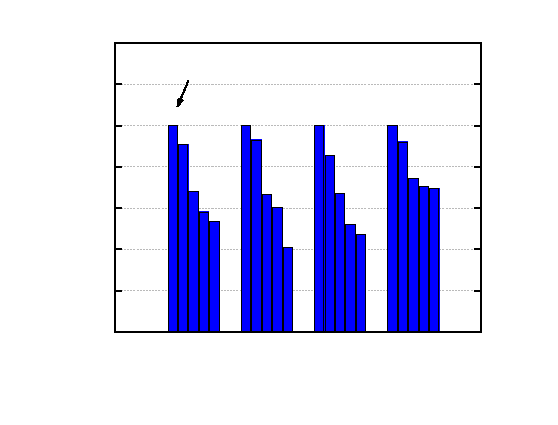
\includegraphics{parallel-ancestor-build}}%
    \gplfronttext
  \end{picture}%
\endgroup

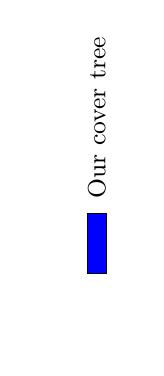
\begin{tikzpicture}
    \node[draw,fill=blue,minimum width=0.05in,minimum height=0.3in] at (0.3in,0) {};
    \node at (0.3in,0.63in) {\small\rotatebox{90}{Our cover tree}};
    \node[minimum width=0.05in,minimum height=0.3in] at (0.45in,0) {};
    \node at (0.45in,0.61in) {\small\rotatebox{90}{}};
    \node at (0,-0.475in) {};
\end{tikzpicture}
\end{center}

\vspace{0.1in}
Experiments run on an Amazon AWS instance with 16 true cores
\end{frame}

%%%%%%%%%%%%%%%%%%%%%%%%%%%%%%%%%%%%%%%%%%%%%%%%%%%%%%%%%%%%%%%%%%%%%%%%%%%%%%%%

\begin{frame}[fragile]{Parallel tree construction really matters on larger data sets}


%on small datasets with cheap metrics, parallel construction is less useful

\vspace{0.1in}
On large datasets with an expensive metric, parallelism is more useful

\vspace{0.15in}
Yahoo! Flickr dataset with 1.5 million images and earth mover distance

%\vspace{0.2in}
\vspace{0.15in}
\begin{center}
\Large
\begin{tabular}{ccccc}
\hline
num cores
 & \multicolumn{2}{c}{simplified tree} & \multicolumn{2}{c}{nearest ancestor tree} \\
%& \multicolumn{2}{c}{construction} & \multicolumn{2}{c}{construction} \\ %\cline{2-5}
& time & speedup & time & speedup \\
\hline
\hline
1  & 70.7 min & 1.0 & 210.9 min& 1.0\\
2  & 36.6 min & 1.9 & 94.2 min & 2.2\\
4  & 18.5 min & 3.8 & 48.5 min & 4.3\\
8  & 10.2 min & 6.9 & 25.3 min & 8.3\\
16 & 6.7 min & 10.5 & 12.0 min & 17.6\\
\hline
\end{tabular}
\end{center}

\end{frame}

%%%%%%%%%%%%%%%%%%%%%%%%%%%%%%%%%%%%%%%%%%%%%%%%%%%%%%%%%%%%%%%%%%%%%%%%%%%%%%%%

\begin{frame}[fragile]{The effect of parallel tree \emph{construction and query}}
\begin{center}
\graphicspath{{slides/paperimg/}}
% GNUPLOT: LaTeX picture with Postscript
\begingroup
  \makeatletter
  \providecommand\color[2][]{%
    \GenericError{(gnuplot) \space\space\space\@spaces}{%
      Package color not loaded in conjunction with
      terminal option `colourtext'%
    }{See the gnuplot documentation for explanation.%
    }{Either use 'blacktext' in gnuplot or load the package
      color.sty in LaTeX.}%
    \renewcommand\color[2][]{}%
  }%
  \providecommand\includegraphics[2][]{%
    \GenericError{(gnuplot) \space\space\space\@spaces}{%
      Package graphicx or graphics not loaded%
    }{See the gnuplot documentation for explanation.%
    }{The gnuplot epslatex terminal needs graphicx.sty or graphics.sty.}%
    \renewcommand\includegraphics[2][]{}%
  }%
  \providecommand\rotatebox[2]{#2}%
  \@ifundefined{ifGPcolor}{%
    \newif\ifGPcolor
    \GPcolortrue
  }{}%
  \@ifundefined{ifGPblacktext}{%
    \newif\ifGPblacktext
    \GPblacktextfalse
  }{}%
  % define a \g@addto@macro without @ in the name:
  \let\gplgaddtomacro\g@addto@macro
  % define empty templates for all commands taking text:
  \gdef\gplbacktext{}%
  \gdef\gplfronttext{}%
  \makeatother
  \ifGPblacktext
    % no textcolor at all
    \def\colorrgb#1{}%
    \def\colorgray#1{}%
  \else
    % gray or color?
    \ifGPcolor
      \def\colorrgb#1{\color[rgb]{#1}}%
      \def\colorgray#1{\color[gray]{#1}}%
      \expandafter\def\csname LTw\endcsname{\color{white}}%
      \expandafter\def\csname LTb\endcsname{\color{black}}%
      \expandafter\def\csname LTa\endcsname{\color{black}}%
      \expandafter\def\csname LT0\endcsname{\color[rgb]{1,0,0}}%
      \expandafter\def\csname LT1\endcsname{\color[rgb]{0,1,0}}%
      \expandafter\def\csname LT2\endcsname{\color[rgb]{0,0,1}}%
      \expandafter\def\csname LT3\endcsname{\color[rgb]{1,0,1}}%
      \expandafter\def\csname LT4\endcsname{\color[rgb]{0,1,1}}%
      \expandafter\def\csname LT5\endcsname{\color[rgb]{1,1,0}}%
      \expandafter\def\csname LT6\endcsname{\color[rgb]{0,0,0}}%
      \expandafter\def\csname LT7\endcsname{\color[rgb]{1,0.3,0}}%
      \expandafter\def\csname LT8\endcsname{\color[rgb]{0.5,0.5,0.5}}%
    \else
      % gray
      \def\colorrgb#1{\color{black}}%
      \def\colorgray#1{\color[gray]{#1}}%
      \expandafter\def\csname LTw\endcsname{\color{white}}%
      \expandafter\def\csname LTb\endcsname{\color{black}}%
      \expandafter\def\csname LTa\endcsname{\color{black}}%
      \expandafter\def\csname LT0\endcsname{\color{black}}%
      \expandafter\def\csname LT1\endcsname{\color{black}}%
      \expandafter\def\csname LT2\endcsname{\color{black}}%
      \expandafter\def\csname LT3\endcsname{\color{black}}%
      \expandafter\def\csname LT4\endcsname{\color{black}}%
      \expandafter\def\csname LT5\endcsname{\color{black}}%
      \expandafter\def\csname LT6\endcsname{\color{black}}%
      \expandafter\def\csname LT7\endcsname{\color{black}}%
      \expandafter\def\csname LT8\endcsname{\color{black}}%
    \fi
  \fi
  \setlength{\unitlength}{0.0500bp}%
  \begin{picture}(5040.00,3772.00)%
    \gplgaddtomacro\gplbacktext{%
      \csname LTb\endcsname%
      \put(1254,1129){\makebox(0,0)[r]{\strut{}$2^{-4}$}}%
      \csname LTb\endcsname%
      \put(1254,1526){\makebox(0,0)[r]{\strut{}$2^{-3}$}}%
      \csname LTb\endcsname%
      \put(1254,1922){\makebox(0,0)[r]{\strut{}$2^{-2}$}}%
      \csname LTb\endcsname%
      \put(1254,2318){\makebox(0,0)[r]{\strut{}$2^{-1}$}}%
      \csname LTb\endcsname%
      \put(1254,2714){\makebox(0,0)[r]{\strut{}$2^{+0}$}}%
      \csname LTb\endcsname%
      \put(1254,3111){\makebox(0,0)[r]{\strut{}$2^{+1}$}}%
      \put(1873,601){\rotatebox{-45}{\makebox(0,0)[l]{\strut{}yearpredict}}}%
      \put(1873,381){\rotatebox{-45}{\makebox(0,0)[l]{\strut{}(277min)}}}%
      \put(2471,601){\rotatebox{-45}{\makebox(0,0)[l]{\strut{}twitter}}}%
      \put(2471,381){\rotatebox{-45}{\makebox(0,0)[l]{\strut{}(51min)}}}%
      \put(3068,601){\rotatebox{-45}{\makebox(0,0)[l]{\strut{}tinyImages}}}%
      \put(3068,381){\rotatebox{-45}{\makebox(0,0)[l]{\strut{}(34min)}}}%
      \put(3666,601){\rotatebox{-45}{\makebox(0,0)[l]{\strut{}mnist}}}%
      \put(3666,381){\rotatebox{-45}{\makebox(0,0)[l]{\strut{}(30min)}}}%
      \put(176,2120){\rotatebox{-270}{\makebox(0,0){\strut{}normalized total runtime}}}%
      \put(396,2120){\rotatebox{-270}{\makebox(0,0){\strut{}(both \emph{construction} and \emph{query})}}}%
      \put(616,2120){\rotatebox{-270}{\makebox(0,0){\strut{}  }}}%
      \put(1774,2980){\makebox(0,0)[l]{\strut{}\tiny 1}}%
      \put(1849,3174){\makebox(0,0)[l]{\strut{}\tiny 1}}%
      \put(1924,2814){\makebox(0,0)[l]{\strut{}\tiny 1}}%
      \put(1983,2453){\makebox(0,0)[l]{\strut{}\tiny 2}}%
      \put(2058,1954){\makebox(0,0)[l]{\strut{}\tiny 4}}%
      \put(2124,1648){\makebox(0,0)[l]{\strut{}\tiny 8}}%
      \put(2184,1399){\makebox(0,0)[l]{\strut{}\tiny 16}}%
    }%
    \gplgaddtomacro\gplfronttext{%
    }%
    \gplbacktext
    \put(0,0){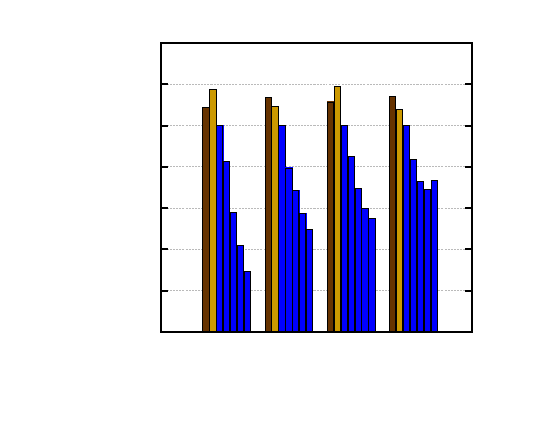
\includegraphics{parallel}}%
    \gplfronttext
  \end{picture}%
\endgroup

\definecolor{colorOrig}{RGB}{102,51,0}
\definecolor{colorMlpack}{RGB}{204,153,0}
\begin{tikzpicture}
    \node[draw,fill=colorOrig,minimum width=0.05in,minimum height=0.3in] at (0,0) {};
    \node at (0,0.79in) {\small\rotatebox{90}{Reference cover tree}};
    \node[draw,fill=colorMlpack,minimum width=0.05in,minimum height=0.3in] at (0.15in,0) {};
    \node at (0.15in,0.80in) {\small\rotatebox{90}{MLPack's cover tree}};
    \node[draw,fill=blue,minimum width=0.05in,minimum height=0.3in] at (0.3in,0) {};
    \node at (0.3in,0.63in) {\small\rotatebox{90}{Our cover tree}};
    \node[minimum width=0.05in,minimum height=0.3in] at (0.45in,0) {};
    \node at (0.45in,0.61in) {\small\rotatebox{90}{}};
    \node at (0,-0.475in) {};
\end{tikzpicture}
\end{center}

\vspace{0.1in}
Experiments run on an Amazon AWS instance with 16 true cores
\end{frame}


%%%%%%%%%%%%%%%%%%%%%%%%%%%%%%%%%%%%%%%%

\begin{frame}{Summary}

\Large

You should use cover trees.

\vspace{0.35in}
We made them easier to implement and faster.

\vspace{0.35in}
%\rule{\textwidth}{1pt}
%\vspace{-0.10in}

All the code is licensed under the BSD3 and available at:

\begin{center}
\url{http://github.com/mikeizbicki/hlearn}
\end{center}

%It's written in Haskell.

\end{frame}

%%%%%%%%%%%%%%%%%%%%%%%%%%%%%%%%%%%%%%%%%%%%%%%%%%%%%%%%%%%%%%%%%%%%%%%%%%%%%%%


\end{document}



